\documentclass[11pt]{article}
\usepackage{amssymb,amsmath,amsthm}
\usepackage{verbatim}
\usepackage{fullpage}
\usepackage{gencor}
\usepackage{mathrsfs}
\usepackage{authblk}
\usepackage{graphicx}
\usepackage{caption}
\usepackage{cite}
\usepackage{subcaption}
\usepackage{mathtools}
\usepackage{multirow}
\usepackage[nottoc,notlof,notlot,numbib]{tocbibind}
\usepackage{xr-hyper}
\externaldocument[supp-]{supp}
\renewcommand*{\fnsymbol}[1]{\ensuremath{\ifcase#1\or *\or**\or\dagger\or \ddagger\or
   \mathsection\or \mathparagraph\or \|\or **\or \dagger\dagger
   \or \ddagger\ddagger \else\@ctrerr\fi}}
 \newcommand{\beginsupplement}{%
        \setcounter{table}{0}
        \renewcommand{\thetable}{S\arabic{table}}%
        \setcounter{figure}{0}
        \renewcommand{\thefigure}{S\arabic{figure}}%
     }

\makeatother

\frenchspacing
\title{An Atlas of Genetic Correlations across Human Diseases and Traits}
\author[1,2,3]{Brendan Bulik-Sullivan$^{\ddagger,}$\thanks{Co-first authors}$^,$}
\author[*,4]{Hilary K Finucane$^{\ddagger,}$}
\author[1,2,3]{Verneri Anttila}
\author[5,6]{Alexander Gusev}
\author[7]{Felix R. Day}
\author[1,5]{Po-Ru Loh}
\author[8]{ReproGen Consortium}
\author[8]{Psychiatric Genomics Consortium}
\author[8]{Genetic Consortium for Anorexia Nervosa of the Wellcome Trust Case Control Consortium 3}
\author[1,2,3]{Laramie Duncan}
\author[7]{John R.B. Perry}
\author[1]{Nick Patterson}
\author[1,2,3]{Elise B. Robinson}
\author[1,2,3]{Mark J. Daly}
\author[1,5,6]{Alkes L. Price\thanks{Co-last authors}$^,$$^{\ddagger,}$}
\author[,1,2,3]{Benjamin M. Neale$^{\dagger,}$\thanks{Address correspondence to BBS (\texttt{bulik@broadinstitute.org}), BMN (\texttt{bneale@broadinstitute.org}), HKF (\texttt{hilaryf@mit.edu}) and ALP (\texttt{aprice@hsph.harvard.edu}).}}

\affil[1]{\small{Program in Medical and Population Genetics, Broad Institute of MIT and Harvard, Cambridge, MA, USA}}
\affil[2]{Stanley Center for Psychiatric Genetics, Broad Institute of MIT and Harvard, Cambridge, MA, USA}
\affil[3]{Analytic and Translational Genetics Unit, Massachusetts General Hospital and Harvard Medical School, Boston, Massachusetts, USA.}
\affil[4]{Department of Mathematics, Massachusetts Institute of Technology, Cambridge, MA, USA.}
\affil[5]{Department of Epidemiology, Harvard T.H. Chan School of Public Health, Boston, MA, USA.}
\affil[6]{Department of Biostatistics, Harvard T.H. Chan School of Public Health, Boston, MA, USA.}
\affil[7]{MRC Epidemiology Unit, University of Cambridge School of Clinical Medicine, Institute of Metabolic Science, Cambridge Biomedical Campus, Cambridge, CB2 0QQ, UK}
\affil[8]{A list of members and affiliations appears in the Supplementary Note.}
\date{}
\begin{document}
\maketitle

\begin{abstract}
Identifying genetic correlations between complex traits and diseases can provide useful etiological insights and help prioritize likely causal relationships.
The major challenges preventing estimation of genetic correlation from genome-wide association study (GWAS) data with current methods are the lack of availability of individual genotype data and widespread sample overlap among meta-analyses.
We circumvent these difficulties by introducing a technique -- cross-trait LD Score regression -- for estimating genetic correlation that requires only GWAS summary statistics and is not biased by sample overlap.
We use this method to estimate 276 genetic correlations among 24 traits.
The results include genetic correlations between anorexia nervosa and schizophrenia, anorexia and obesity and associations between educational attainment and several diseases.
These results highlight the power of genome-wide analyses, since there currently are no genome-wide significant SNPs for anorexia nervosa and only three for educational attainment. 
 
\end{abstract}
\newpage
%%%%%%%%%%%%%%%%%%%%%%%%%%%%%%%%%%%%%%%%%%%%%%%%%%%%%%%%%%%%%%%
\section*{Introduction}
\label{Introduction}
%%%%%%%%%%%%%%%%%%%%%%%%%%%%%%%%%%%%%%%%%%%%%%%%%%%%%%%%%%%%%%%

Understanding the complex relationships among human traits and diseases is a fundamental goal of epidemiology. 
Randomized controlled trials and longitudinal studies are time-consuming and expensive, so
many potential risk factors are studied using cross-sectional correlations studies at a single time point. 
Obtaining causal inferences from such studies can be challenging due
to issues such as confounding and reverse causation, which can lead to spurious associations and mask the effects of real risk factors \cite{smith2003mendelian, smith2014mendelian}. 
Genetics can help elucidate cause and effect, since inherited genetic risks cannot be subject to reverse causation and are correlated with a smaller list of confounders.

The first methods for testing for genetic overlap were family studies \cite{vandenberg1965multivariate, 
kempthorne1961interpretation,
loehlin1966genetic,
neale1992methodology,
lichtenstein2009common}.
In order to estimate genetic overlaps among many pairs of phenotypes, family designs require measuring multiple traits on the same individuals.
Consequently, it is challenging to scale family designs to a large number of traits,
espqecially traits that difficult or costly to measure (\emph{e.g.,} low-prevalence diseases).
More recently, genome-wide association studies (GWAS) have allowed us to obtain effect-size estimates for specific genetic variants, 
so it is possible to test for shared genetics by looking for correlations in effect-sizes across traits, 
which does not require measuring multiple traits per individual.

There exists a large class of methods for interrogating genetic overlap via GWAS that focus only on genome-wide significant SNPs. 
One of the most influential methods in this class is Mendelian randomization, which uses
significantly associated SNPs as instrumental variables to attempt quantify causal relationships between risk factors and disease\cite{smith2003mendelian, smith2014mendelian}. 
Methods that focus on significant SNPs are effective for traits where there are many
significant associations that account for a substantial fraction of heritability \cite{voight2012plasma,do2013common}.
For many complex traits, heritability is distributed over thousands of variants with small effects, 
and the proportion of heritability accounted for by significantly associated variants at current sample sizes is small \cite{visscher2012five}.
In such situations, one can often obtain more accurate results by using genome-wide data, rather than just significantly associated variants \cite{yang2010}.

A complementary approach is to estimate genetic correlation, which includes the effects of all SNPs,
including those that do not reach genome-wide significance (Methods).
The two main existing techniques for estimating genetic correlation from GWAS data are restricted maximum likelihood (REML) \cite{yang2010, yang2011gcta, lee2012estimation, pgccdg2013, vattikuti2012heritability, chen2014estimation}
and polygenic scores \cite{purcell2009common, dudbridge2013power}.
These methods have only been applied to a few traits, 
because they require individual genotype data, 	
which are difficult to obtain due to informed consent limitations. 

In order to overcome these limitations, we have developed a technique for estimating genetic correlation using only GWAS summary statistics that is not biased by sample overlap.
Our method, cross-trait LD Score regression, is a simple extension of single-trait LD Score regression \cite{buliksullivan2014} and is computationally very fast.
We apply this method to data from 24 GWAS and report genetic correlations for 276 pairs of phenotypes, demonstrating shared genetic bases for many complex diseases and traits.  

%%%%%%%%%%%%%%%%%%%%%%%%%%%%%%%%%%%%%%%%%%%%%%%%%%%%%%%%%%%%%%%
\section*{Results}\label{Results}
%%%%%%%%%%%%%%%%%%%%%%%%%%%%%%%%%%%%%%%%%%%%%%%%%%%%%%%%%%%%%%%

\subsection*{Overview of Methods}

The method presented here for estimating genetic correlation from summary statistics relies on the fact that the GWAS effect-size estimate for a given SNP incorporates the effects of all SNPs in linkage disequilibrium (LD) with that SNP \cite{yang2011genomic,buliksullivan2014}. 
For a polygenic trait, SNPs with high LD will have higher $\chi^2$ statistics on average than SNPs with low LD \cite{buliksullivan2014}. 
A similar relationship holds if we replace $\chi^2$ statistics for a single study with the product of $z$-scores from two studies of traits with non-zero genetic correlation. 

More precisely, under a polygenic model \cite{yang2010,lee2012estimation}, the expected value of $z_{1j}z_{2j}$ is 
\begin{equation}\label{reg_eqn}
	\E[z_{1j}z_{2j}] = \dfrac{\sqrt{N_1N_2}\rho_g}{M}\ell_j + \dfrac{\rho N_s}{\sqrt{N_1N_2}},
\end{equation}
where $N_i$ is the sample size for study $i$, $\rho_g$ is genetic covariance (defined in Methods), $\ell_j$ is LD Score \cite{buliksullivan2014}, $N_s$ is the number of individuals included in both studies, and $\rho$ is the phenotypic correlation among the $N_s$ overlapping samples.
We derive this equation in the Supplementary Note.
If study 1 and study 2 are the same study, then Equation \ref{reg_eqn} reduces to the single-trait result from \cite{buliksullivan2014}, 
because genetic covariance between a trait and itself is heritability, and $\chi^2 = z^2$.
As a consequence of equation 1, we can estimate genetic covariance using the slope from the regression of $z_{1j}z_{2j}$ on LD Score, which is computationally very fast (Methods). 

Sample overlap creates spurious correlation between $z_{1j}$ and $z_{2j}$, which inflates $z_{1j}z_{2j}$.
The expected magnitude of this inflation is uniform across all markers, and in particular does not depend on LD Score.
As a result, sample overlap only affects the intercept from this regression (the term $\rho N_s/\sqrt{N_1N_2}$) and not the slope,
so the estimates of genetic correlation will not be biased by sample overlap.
Similarly, shared population stratification will alter the intercept but have minimal impact on the slope, 
because the correlation between LD Score and the rate of genetic drift is minimal \cite{buliksullivan2014}.
If we are willing to assume no shared population stratification, and 
we know the amount of sample overlap and phenotypic correlation in advance (\emph{i.e.,} the true value of $\rho N_s/\sqrt{N_1N_2}$), 
we can constrain the intercept to this value.
We refer to this approach as constrained intercept LD Score regression.
Constrained intercept LD Score regression has lower standard error -- often by as much as 30\% -- than LD Score regression with unconstrained intercept, but will yield biased and misleading estimates if the intercept is misspecified, \emph{e.g.,} if we miscount the overlapping samples or do not control for population stratification.

Normalizing genetic covariance by the SNP-heritabilities yields genetic correlation: 
$r_g \coloneqq\rho_g/\sqrt{h^2_1h^2_2},$ where $h^2_i$ denotes the SNP-heritability \cite{yang2010} from study $i$.
Genetic correlation ranges between $-1$ and $1$.
Results similar to Equation \ref{reg_eqn} hold if one or both studies is a case/control study, in which case genetic covariance is on the observed scale.
Details are provided in the Supplementary Note.
There is no distinction between observed and liability scale genetic correlation for case/control traits, so we can talk about 
genetic correlation between a case/control trait and a quantitative trait and genetic correlation between pairs of case/control traits without the need to specify a scale (Supplementary Note).


\subsection*{Simulations}\label{Simulations}
We performed a series of simulations to evaluate the robustness of the model to potential confounders such as sample overlap
and model misspecification, and to verify the accuracy of the standard error estimates (Methods).

Table \ref{main_simulations} shows cross-trait LD Score regression estimates and standard errors from 1,000 simulations of quantitative traits.
For each simulation replicate, 
we generated two phenotypes for each of 2,062 individuals in our sample by drawing effect sizes approximately 600,000 SNPs on chromosome 2 from a bivariate normal distribution.
We then computed summary statistics for both phenotypes and estimated heritability and genetic correlation with cross-trait LD Score regression.
The summary statistics were generated from completely overlapping samples.
Results are shown in Table \ref{main_simulations}.
These simulations confirm that cross-trait LD Score regression yields accurate estimates of the true genetic correlation
and that the standard errors match the standard deviation across simulations. 
Thus, cross-trait LD Score regression is not biased by sample overlap, 
in contrast to estimation of genetic correlation via polygenic risk scores, which is biased in the presence of sample overlap \cite{dudbridge2013power}. 
We also evaluated simulations with one quantitative trait and one case/control study and show that cross-trait LD Score regression can be applied to binary traits 
and is not biased by oversampling of cases (Table  \ref{qt_cc}).

\begin{table}[ht]
\centering
\begin{tabular}{rrrrr}
  \hline
Parameter & Truth & Estimate & SD & SE \\
  \hline
$h^2$ & 0.58 & 0.58 & 0.072 & 0.075 \\
$\rho_g$ & 0.29 & 0.29 & 0.057 & 0.058 \\
  $r_g$ & 0.50 & 0.49 & 0.079 & 0.073 \\
   \hline
\end{tabular}
\caption{\label{main_simulations}\small{Simulations with complete sample overlap. Truth shows the true parameter values.
Estimate shows the average cross-trait LD Score regression estimate across 1000 simulations. SD shows the standard deviation of the estimates across 1000 simulations, and SE shows the mean cross-trait LD Score regression SE across 1000 simulations. Further details of the simulation setup are given in the Methods.}}
\end{table}

Estimates of heritability and genetic covariance can be biased if the underlying model of genetic architecture is misspecified, \emph{e.g.,} if variance explained is correlated with LD Score or MAF \cite{speed2012improved, buliksullivan2014}.
Because genetic correlation is estimated as a ratio, it is more robust;
biases that affect the numerator and the denominator in the same direction tend to cancel. 
We obtain approximately correct estimates of genetic correlation even in simulations with models of genetic architecture where our estimates of heritability and genetic covariance are biased (Table \ref{parallel}).

\subsection*{Replication of Pyschiatric Cross-Disorder Results}\label{PGCCDG}
As technical validation, we replicated the estimates of genetic correlations among psychiatric disorders obtained with individual genotypes and REML in \cite{pgccdg2013}, 
by applying cross-trait LD Score regression to summary statistics from the same data \cite{cross2013identification}.
These summary statistics were generated from non-overlapping samples, so
we applied cross-trait LD Score regression using both unconstrained and constrained intercepts (Methods).
Results from these analyses are shown in Figure \ref{Fig:Replication of PGC Cross-Disorder Results}.
The results from cross-trait LD Score regression were similar to the results from REML.
cross-trait LD Score regression with constrained intercept gave standard errors that were only slightly larger than those from REML,
while the standard errors from cross-trait LD Score regression with intercept were substantially larger, 
especially for traits with small sample sizes (\emph{e.g.,} ADHD, ASD).

% Figure 1 -- replication of PGC-CDG results
\begin{figure}[!ht]
\begin{centering}
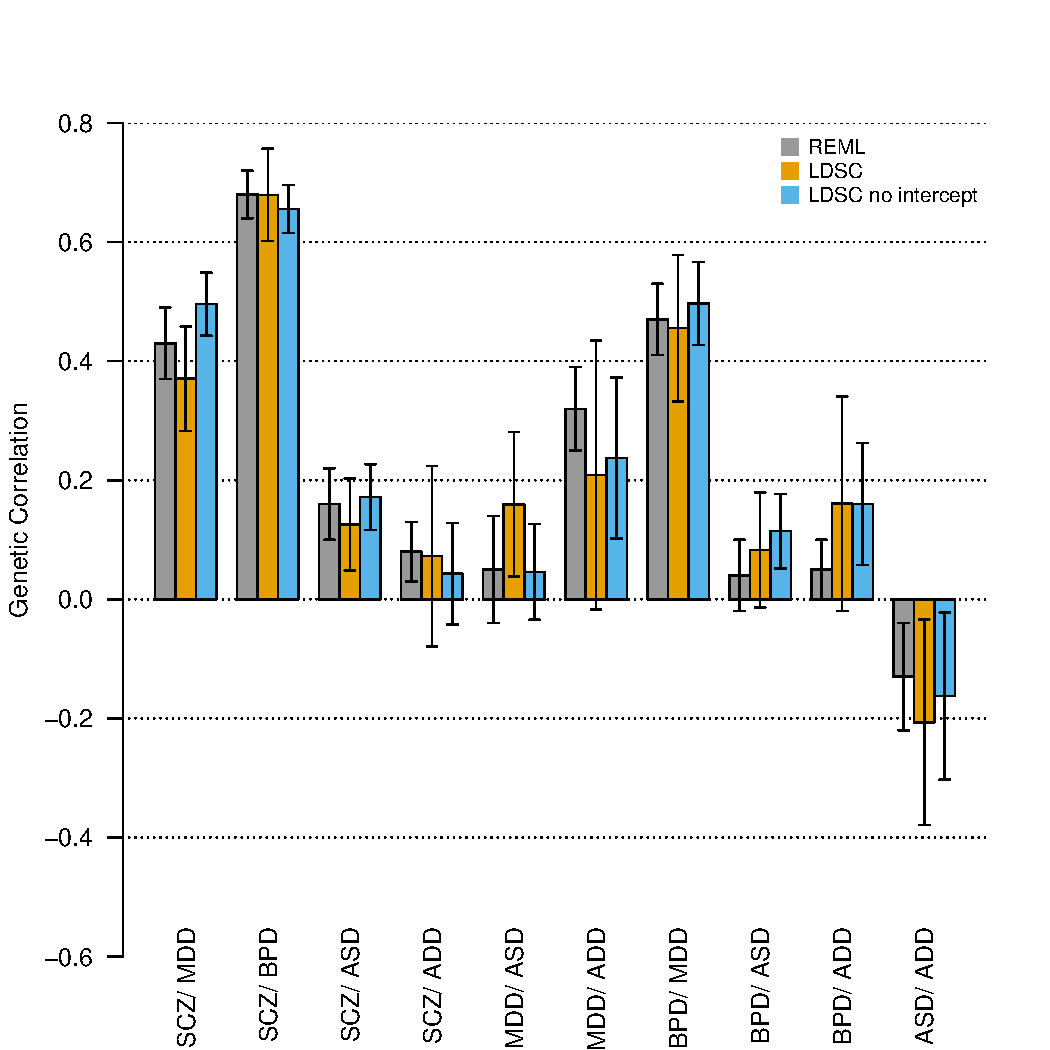
\includegraphics[scale=0.9]{figs/ldsc_vs_gcta.pdf}
\end{centering}
\caption{\label{Fig:Replication of PGC Cross-Disorder Results}\small{Replication of Psychiatric Cross-Disorder Results.
This plot compares cross-trait LD Score regression estimates of genetic correlation using the summary statistics from \cite{cross2013identification} to estimates obtained from REML with the same data \cite{pgccdg2013}.
The horizontal axis indicates pairs of phenotypes, 
and the vertical axis indicates genetic correlation.
Error bars are standard errors.
Green is REML; orange is LD Score with intercept and white is LD Score with constrained intercept.
The estimates of genetic correlation among psychiatric phenotypes in figure \ref{Fig:300 Gencors} use larger sample sizes;
this analysis is intended as a technical validation.
Abbreviations: 
ADHD = attention deficit disorder;
ASD = autism spectrum disorder;
BPD = bipolar disorder;
MDD = major depressive disorder;
SCZ = schizophrenia.}}
\end{figure}

\subsection*{Application to Summary Statistics From 25 Phenotypes}

We used cross-trait LD Score regression to estimate genetic correlations among 24 phenotypes (URLs, Methods).
Genetic correlation estimates for all 276 pairwise combinations of the 24 traits are shown in Figure \ref{Fig:300 Gencors}.
For clarity of presentation, 
the 24 phenotypes were restricted to contain only one phenotype from each cluster of closely related phenotypes (Methods).
Genetic correlations among the educational, anthropometric, smoking, and insulin-related phenotypes that were excluded from Figure \ref{Fig:300 Gencors}
are shown Supplementary Figures \ref{edu}, and \ref{giant}, \ref{smoking} and \ref{insulin}, respectively.
A full table of 1176 genetic correlations among 49 traits is provided in Supplementary Table S4.
References and sample sizes are shown in Supplementary Table \ref{N}.

% Figure 2 -- Genetic correlation heatmap with 25 traits
\begin{figure}[!ht]
\begin{centering}
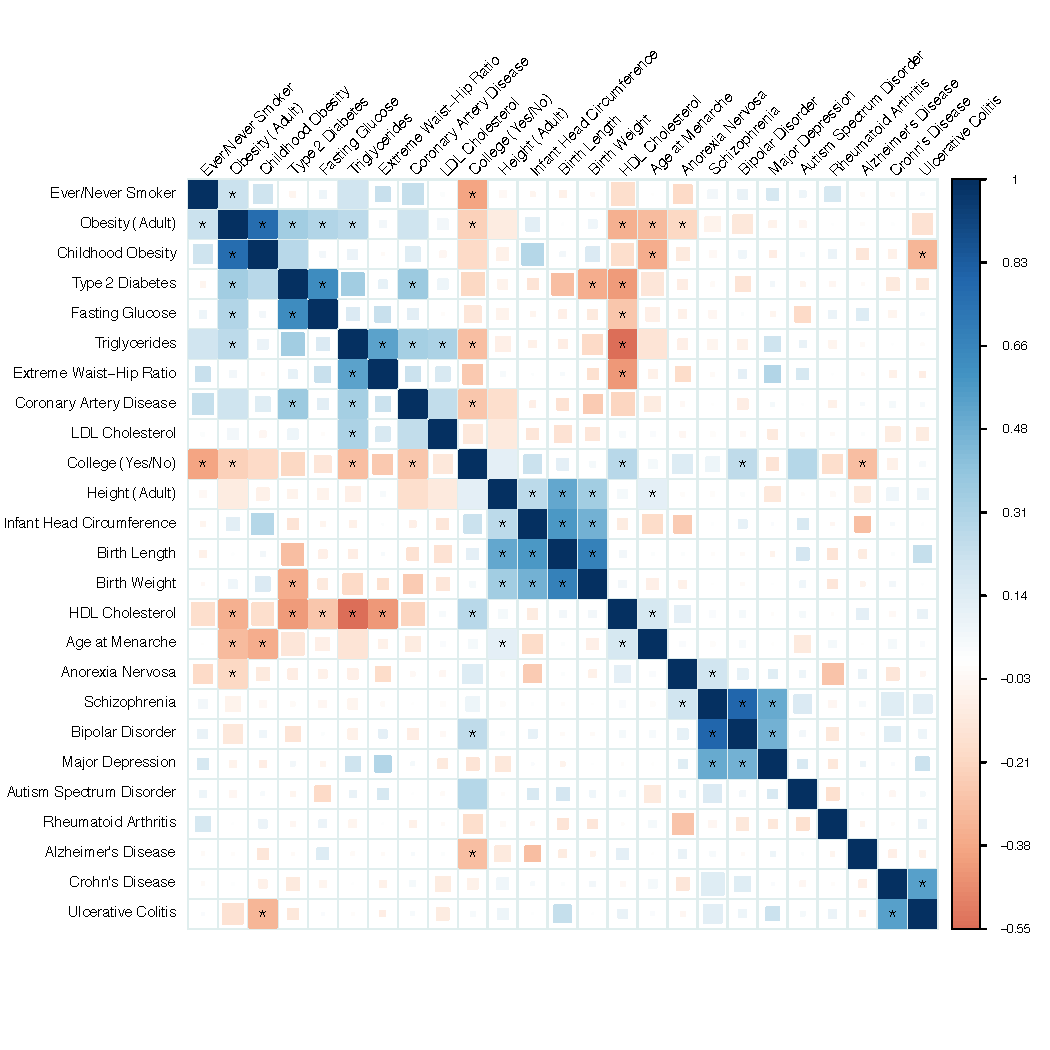
\includegraphics[scale=0.9]{figs/rg_heatmap.pdf}

\caption{         
\label{Fig:300 Gencors}
\small{Genetic Correlations among 24 GWAS.
Blue represents positive genetic correlations; red represents negative. 
Larger squares correspond to more significant $p$-values.
Genetic correlations that are different from zero at 1\% FDR are shown as full-sized squares. 
Genetic correlations that are significantly different from zero after Bonferroni correction for the 300 tests in this figure have an asterisk. 
We show results that do not pass multiple testing correction as smaller squares in order to avoid whiting out positive controls 
where the estimate points in the expected direction, but does not achieve statistical significance due to small sample size.
This multiple testing correction is conservative, since the tests are not independent.
In order to keep this figure to a reasonable size, we have picked representatives of several clusters of highly correlated traits.
Additional genetic correlations can be found in Supplementary Figures \ref{edu}, \ref{giant}, \ref{smoking} and \ref {insulin}.
All genetic correlations in this paper can be found in tabular form in Supplementary Table S4.
}}
\end{centering}
\end{figure}

% Results that are consistent with top SNP results or MR analyses 
For the majority of pairs of traits in Figure \ref{Fig:300 Gencors}, no GWAS-based genetic correlation estimate has been reported; 
however, many associations have been described informally based on the observation of overlap among genome-wide significant loci.
Examples of genetic correlations that are consistent with overlap among top loci include the correlations between plasma lipids and cardiovascular disease \cite{do2013common}; age at onset of menarche and obesity \cite{perry2014parent}; type 2 diabetes, obesity, fasting glucose, plasma lipids and cardiovascular disease \cite{morris2012large}; birth weight, adult height and type 2 diabetes \cite{horikoshi2013new, freathy2009type}; birth length, adult height and infant head circumference \cite{early2012genome, taal2012common}; and childhood obesity and adult obesity \cite{early2012genome}. 
For many of these pairs of traits, we can reject the null hypothesis of zero genetic correlation with overwhelming statistical
significance (\emph{e.g.,} $p<10^{-20}$ for age at onset of menarche and BMI).

% Table 1 -- interesting genetic correlation results highlighted in the main text
\begin{table}[h!]
\centering
\begin{tabular}{ l|llll}
 & Phenotype 1 & Phenotype 2 & $r_g$ (se) & $p$-value \\
\hline
\multirow{13}{*}{Epidemiological} 
& Age at Menarche & Height (Adult) & 0.13 (0.03) & $2\times10^{-6\ **}$  \\
& Age at Menarche & Type 2 Diabetes & -0.13 (0.04) & $2\times10^{-3\ *}$  \\
& Age at Menarche & Triglycerides & -0.12 (0.04) & $1\times10^{-3\ *}$ \\
& Coronary Artery Disease & Age at Menarche &  -0.12 (0.05) & $3\times10^{-2}$ \\
& Coronary Artery Disease & Years of Education & -0.25 (0.06) & $1\times10^{-4\ **}$ \\
& Coronary Artery Disease & Height (Adult) &  -0.17 (0.04) & $1\times10^{-5\ **}$\\
& Alzheimer's & Years of Education & -0.29 (0.1) & $5\times10^{-3\ *}$ \\
& Bipolar Disorder & Years of Education & 0.30 (0.06) & $9\times10^{-7\ **}$ \\
& BMI & Years of Education & -0.28 (0.03) & $6\times10^{-16\ **}$\\
& Triglycerides & Years of Education & -0.26 (0.06)& $2\times10^{-8\ **}$ \\
& Anorexia Nervosa & BMI & -0.18 (0.04) & $3\times10^{-7\ **}$ \\
& Ever/Never Smoker & Years of Education & -0.36 (0.06) & $2\times10^{-8\ **}$ \\
& Ever/Never Smoker & BMI & 0.20 (0.04) & $8\times10^{-7\ **}$ \\
\hline
\multirow{3}{*}{New/Nonzero} 
& Autism Spectrum Disorder & Years of Education & 0.30 (0.08) & $2\times10^{-4\ *}$\\
& Ulcerative Colitis & Childhood Obesity & -0.34 (0.08) & $3.1\times10^{-5\ **}$\\
& Anorexia Nervosa & Schizophrenia & 0.19 (0.04)  & $2\times10^{-5\ **}$ \\
\hline
\multirow{8}{*}{New/Low} 
& Schizophrenia &Alzheimer's &  0.04 (0.06) & 0.58 \\
& Schizophrenia & Ever/Never Smoker & 0.05 (0.05) & 0.26 \\
& Schizophrenia & Triglycerides & -0.04 (0.04) & 0.29 \\
& Schizophrenia & LDL Cholesterol & -0.01 (0.04) & 0.72 \\
& Schizophrenia & HDL Cholesterol & 0.03 (0.04) & 0.49 \\
& Schizophrenia & Rheumatoid Arthritis & -0.04 (0.05) & 0.39 \\
& Crohn's Disease & Rheumatoid Arthritis & -0.03 (0.08) & 0.73 \\
& Ulcerative Colitis & Rheumatoid Arthritis & 0.09 (0.08) & 0.30 \\
\end{tabular}
\caption{
\small{\label{table:results}Genetic correlation estimates, standard errors and $p$-values for selected pairs of traits. Results are grouped into
 genetic correlations that are new genetic results, but are consistent with established epidemiological associations (``Epidemiological''), genetic correlations that are new both to genetics and epidemiology (``New/Nonzero'') and interesting null results (``New/Low''). 
The $p$-values are uncorrected $p$-values.
Results that pass multiple testing correction for the 300 tests in Figure \ref{Fig:300 Gencors} at 1\% FDR have a single asterisk; results that pass Bonferroni correction have two asterisks.
We present some genetic correlations that agree with epidemiological associations but that do not pass multiple testing correction in these data. }}
\end{table}

% Novel genetic results that are not novel epidemiological results
The first section of Table \ref{table:results} lists genetic correlation results that are consistent with epidemiological associations, 
but, as far as we are aware, have not previously been reported using genetic data.
The estimates of the genetic correlation between age at onset of menarche and adult height \cite{onland2005age}, triglycerides \cite{day2014} and type 2 diabetes \cite{day2014, elks2013age} are consistent with the epidemiological associations. 
The estimate of a negative genetic correlation between anorexia nervosa and obesity suggests that the same genetic factors influence normal variation in BMI as well as dysregulated BMI in psychiatric illness.
This result is consistent with the observation that BMI GWAS findings implicate neuronal, rather than metabolic, cell-types and epigenetic marks 
\cite{finucane2014partitioning, farooqi2014defining}.
The negative genetic correlation between adult height and coronary artery disease agrees with a replicated epidemiological association  \cite{wang2011associations,hebert1993height,rich1995height}.
We observe several significant associations with the educational attainment phenotypes from
Rietveld \emph{et al.} \cite{rietveld2013gwas}:
we estimate a statistically significant negative genetic correlation between college and Alzheimer's disease, 
which agrees with epidemiological results \cite{barnes2011projected, norton2014potential}. 
The positive genetic correlation between college and bipolar disorder is consistent with previous epidemiological reports \cite{maccabe2010excellent, tiihonen2005premorbid}.
The estimate of a negative genetic correlation between smoking and college is consistent with the observed differences in smoking rates as a function of educational attainment  \cite{pierce1989trends}.

% Novel results
The second section of table \ref{table:results} lists three results that are, to the best of our knowledge, new both to genetics and epidemiology.
One, we find a positive genetic correlation between anorexia nervosa and schizophrenia.
Comorbidity between eating and psychotic disorders has not been thoroughly investigated in the psychiatric literature \cite{striegel1999psychiatric,blinder2006psychiatric}, and this result raises the possibility of  similarity between these classes of disease.
Two, we estimate a negative genetic correlation between ulcerative colitis (UC) and childhood obesity.
The relationship between premorbid BMI and ulcerative colitis is not well-understood; exploring this relationship may be a fruitful direction for further investigation. 
Three, we estimate a positive genetic correlation between autism spectrum disorder (ASD) and educational attainment (
which has very high genetic correlation with IQ \cite{deary2007intelligence, calvin2010sex, rietveld2013gwas}).
The ASD summary statistics were generated using a case-pseudocontrol study design, so this result cannot be explained by oversampling of ASD cases from the more highly educated parents, which is observed epidemiologically \cite{durkin2010socioeconomic}. 
The distribution of IQ among individuals with ASD has lower mean than the general population, but with heavy tails \cite{robinson2014autism} (\emph{i.e.,} an excess of individuals with low and high IQ).
There is also emerging evidence that the genetic architecture of ASD varies across the IQ distribution \cite{samocha2014framework}.

% Interesting null results
The third section of table \ref{table:results} lists interesting examples where the genetic correlation is close to zero with small standard error.
The low genetic correlation between schizophrenia and rheumatoid arthritis is interesting because schizophrenia has been observed to be protective for rheumatoid arthritis \cite{silman2002epidemiology}, though the epidemiological effect is weak, so it is possible that there is a real genetic correlation, but it is too small for us to detect.
The low genetic correlation between schizophrenia and smoking is notable because of the hincreased tobacco use (both prevalence and number of cigarettes per day) among individuals with schizophrenia \cite{de2005meta}. 
The low genetic correlation between schizophrenia and plasma lipid levels contrasts with a previous report of pleiotropy between schizophrenia and triglycerides \cite{andreassen2013improved2}. 
Pleiotropy (unsigned) is different from genetic correlation (signed; see Methods);
however, the pleiotropy reported by Andreassen, \emph{et al.} \cite{andreassen2013improved2} could be explained by the sensitivity of the method used to the properties of a small number of regions with strong LD, rather than trait biology (Figure \ref{qq_tg}).
We estimate near-zero genetic correlation between Alzheimer's disease and schizophrenia. 
The genetic correlations between Alzheimers disease and the other psychiatric traits (anorexia nervosa, bipolar, major depression, ASD) are also
close to zero, but with larger standard errors, due to smaller sample sizes.
This suggests that the genetic basis of Alzheimer's disease is distinct from psychiatric conditions. 
Last, we estimate near zero genetic correlation between rheumatoid arthritis (RA) and both Crohn's disease (CD) and UC. 
Although these diseases share many associated loci \cite{cotsapas2011pervasive,farh2014genetic}, 
there appears to be no directional trend:
some RA risk alleles are also risk alleles for UC and CD, 
but many RA risk alleles are protective for UC and CD \cite{cotsapas2011pervasive}, 
yielding near-zero genetic correlation.
This example highlights the distinction between pleiotropy and genetic correlation (Methods).

Finally, the estimates of genetic correlations among metabolic traits are consistent with the estimates obtained using REML in Vattikuti \emph{et al.}
\cite{vattikuti2012heritability} (Supplementary Table \ref{vattikuti}), and are directionally consistent with the recent Mendelian randomization results from Wuertz \emph{et al.} \cite{wuertz2014metabolic}.
The estimate of 0.54 (0.07) for the genetic correlation between CD and UC is consistent with the estimate of 0.62 (0.04) from Chen \emph{et al.} \cite{chen2014estimation}.

 
%%%%%%%%%%%%%%%%%%%%%%%%%%%%%%%%%%%%%%%%%%%%%%%%%%%%%%%%%%%%%%%
\section*{Discussion}\label{Discussion}
%%%%%%%%%%%%%%%%%%%%%%%%%%%%%%%%%%%%%%%%%%%%%%%%%%%%%%%%%%%%%%%\


% Summary of major findings
We have described a new method for estimating genetic correlation from GWAS summary statistics, which
we applied to a dataset of GWAS summary statistics consisting of 25 traits and more than 1.5 million unique phenotype measurements.
We reported several new findings that would have been difficult to obtain with existing methods, 
including a positive genetic correlation between anorexia nervosa and schizophrenia.
Our method replicated many previously-reported GWAS-based genetic correlations, 
and confirmed observations of overlap among genome-wide significant SNPs, 
MR results and epidemiological associations.

% Importance of findings 
This method is an advance for several reasons: 
it does not require individual genotypes, 
genome-wide significant SNPs or
LD-pruning (which loses information if causal SNPs are in LD).
Our method is not biased by sample overlap and is computationally fast.  
Furthermore, our approach does not require measuring multiple traits on the same individuals, 
so it scales easily to studies of thousands of pairs of traits. 
These advantages allow us to estimate genetic correlation for many more pairs of phenotypes than was possible with existing methods.

% Limitations of Genetic Correlation
The challenges in interpreting genetic correlation are similar to the challenges in MR.
We highlight two difficulties. First,
genetic correlation is immune to environmental confounding, but is subject to genetic confounding, 
analogous to confounding by pleiotropy in MR.
For example, the genetic correlation between HDL and CAD in Figure \ref{Fig:300 Gencors} could result from a causal effect $\mathrm{HDL}\rightarrow\mathrm{CAD}$,
but could also be mediated by triglycerides (TG) \cite{do2013common, burgess2014using}, 
represented graphically \cite{greenland1999causal} as 
$\mathrm{HDL}\leftarrow\mathrm{G}\rightarrow\mathrm{TG}\rightarrow\mathrm{CAD}$, 
where $\mathrm{G}$ is the set of genetic variants with effects on both HDL and TG.
Extending genetic correlation to multiple genetically correlated phenotypes is an important direction for future work \cite{dahl2013network}.
Second, although genetic correlation estimates are not biased by oversampling of cases,
they are affected by other forms of biased sampling, such as misclassification \cite{pgccdg2013}
and case/control/covariate sampling (\emph{e.g.,} a BMI-matched study of T2D).

% Limitations of the Method
We note several limitations of cross-trait LD Score regression as an estimator of genetic correlation.
First, cross-trait LD Score regression requires larger sample sizes than methods that use individual genotypes
in order to achieve equivalent standard error.
Second, cross-trait LD Score regression is not currently applicable to samples from recently-admixed populations.
Third, we have not investigated the potential impact of assortative mating on estimates of genetic correlation, which remains as a future direction.  
Fourth, methods built from polygenic models, such as cross-trait LD Score regression and REML,
are most effective when applied to traits with polygenic genetic architectures. 
For traits where significant SNPs account for a sizable proportion of heritability, analyzing only these SNPs can be more powerful.
Developing methods that make optimal use of both large-effect SNPs and diffuse polygenic signal is a direction for future research.

Despite these limitations, we believe that the cross-trait LD Score regression estimator of genetic correlation will be a useful addition
to the epidemiological toolbox, because it allows for rapid screening for correlations among a diverse set of traits, without the 
need for measuring multiple traits on the same individuals or genome-wide significant SNPs.

\newpage
%%%%%%%%%%%%%%%%%%%%%%%%%%%%%%%%%%%%%%%%%%%%%%%%%%%%%%%%%%%%%%%
\section*{Methods}\label{Methods}
%%%%%%%%%%%%%%%%%%%%%%%%%%%%%%%%%%%%%%%%%%%%%%%%%%%%%%%%%%%%%%%

\subsection*{Definition of Genetic Covariance and Correlation}

All definitions refer to narrow-sense heritabilities and genetic covariances.
Let $S$ denote a set of $M$ SNPs, 
let $X$ denote a vector of additively (0-1-2) coded genotypes for the SNPs in $S$, 
and let $y_1$ and $y_2$ denote phenotypes. Define $\beta \coloneqq  \mathrm{argmax}_{\alpha\in\R^M} \corr\left[y_1, X\alpha\right]$,
where the maximization is performed in the population (\emph{i.e.,} in the infinite data limit). 
Let $\gamma$ denote the corresponding vector for $y_2$.
This is a projection, so $\beta$ is unique modulo SNPs in perfect LD. 
Define $h^2_S$, the heritability explained by SNPs in $S$, as $h^2_S(y_1) \coloneqq  \sum_j \beta_j^2$ and $\rho_S(y_1,y_2)$, the genetic covariance among SNPs in $S$, as
$\rho_S(y_1,y_2) \coloneqq  \sum_{j\in S} \beta_j\gamma_j$.
The genetic correlation among SNPs in $S$ is $r_S(y_1,y_2) \coloneqq  \rho_S(y_1,y_2)/\sqrt{h^2_S(y_1)h^2_S(y_2)}$, 
which lies in [-1,1]. 
Following \cite{yang2010}, we use subscript $g$ (as in $h^2_g,\rho_g,r_g$) when the set of SNPs is 
genotyped and imputed SNPs in GWAS.

SNP genetic correlation ($r_g$) is different from family study genetic correlation.
In a family study, the relationship matrix captures information about all genetic variation, 
not just common SNPs. 
As a result, family studies estimate the total genetic correlation ($S$ equals all variants).
Unlike the relationship between SNP-heritability \cite{yang2010} and total heritability, 
for which $h^2_g \leq h^2$, 
no similar relationship holds between SNP genetic correlation and total genetic correlation.
If $\beta$ and $\gamma$ are more strongly correlated among common variants than rare variants, then the total genetic correlation will be less than the SNP genetic correlation.

Genetic correlation is (asymptotically) proportional to Mendelian randomization estimates.
If we use a genetic instrument $g_i \coloneqq  \sum_{j\in S} X_{ij}\beta_j$ to estimate the effect $b_{12}$ of $y_1$ on $y_2$,
the 2SLS estimate is $\hat{b}_{2SLS}\coloneqq \T{g}y_2/\T{g}y_1$ \cite{angrist2008mostly}.
The expectations of the numerator and denominator are 
$\E[\T{g}y_2]=\rho_S(y_1,y_2)$ and $\E[\T{g}y_1]=h^2_S(y_1)$.
Thus, $\mathrm{plim}_{N\to\infty} \hat{b}_{2SLS} = r_S(y_2,y_1)\sqrt{h^2_S(y_1) / h^2_S(y_2)}$.
If we use the same set $S$ of SNPs to estimate $b_{12}$ and $b_{21}$ (\emph{e.g.,} if $S$ is the set of all common SNPs, as in the genetic correlation analyses in this paper), then this procedure is symmetric in $y_1$ and $y_2$. 

Genetic correlation is different from pleiotropy. 
Two traits have a pleiotropic relationship if many variants affect both.
Genetic correlation is a stronger condition than pleiotropy:
to exhibit genetic correlation, the directions of effect must also be consistently aligned.

%%%%%%%%%%%%%%%%%%%%%%%%%%%%%%%%%%%%%%%%%%%%%%%%%%%%%%%%%%%%%%%
\subsection*{Cross-Trait LD Score Regression} 
%%%%%%%%%%%%%%%%%%%%%%%%%%%%%%%%%%%%%%%%%%%%%%%%%%%%%%%%%%%%%%%


Recall from the Overview of Methods that the cross-trait LD Score regression equation is 

\begin{equation}\label{reg_eqn}
	\E[z_{1j}z_{2j}] = \dfrac{\sqrt{N_1N_2}\rho_g}{M}\ell_j + \dfrac{\rho N_s}{\sqrt{N_1N_2}},
\end{equation}
where $z_{ij}$ denotes the $z$-score for study $i$ and SNP$j$, $N_i$ is the sample size for study $i$, $\rho_g$ is genetic covariance, $\ell_j$ is LD Score \cite{buliksullivan2014}, $N_s$ is the number of individuals included in both studies, and $\rho$ is the phenotypic correlation among the $N_s$ overlapping samples.
We derive this equation in the Supplementary Note.
We estimate genetic covariance by regressing $z_{1j}z_{2j}$ against $\ell_j\sqrt{N_{1j}N_{2j}}$,
(where $N_{ij}$ is the sample size for SNP $j$ in study $i$) 
then multiplying the resulting slope by $M$, the number of SNPs in the reference panel with MAF between 5\% and 50\% 
(technically, this is an estimate of $\pf$, see the Supplementary Note).

If we know the correct value of the intercept term $\rho N_s\sqrt{N_1N_2}$ ahead of time, 
we can reduce the standard error by constraining the intercept to this value using the \texttt{--constrain-intercept} flag in \texttt{ldsc}
(for pairs of binary traits, we give a corresponding expression in terms of the number of overlapping cases and controls in the Supplementary Note).
Note that this works even when there is known nonzero sample overlap 

We recommend using the in-sample estimate of $\rho$ (denoted $\hat{\rho}$), rather than the population value of $\rho$.
Under unbiased sampling $\hat{\rho}$ is consistent for $\rho$ with $\mathcal{O}(1/N)$ variance, 
so in this case, the distinction between $\rho$ and $\hat{\rho}$ is not of great importance.
Under biased sampling (as discussed in the previous section), 
the expected LD Score regression intercept depends on the expected sample correlation 
$\E[y_{i1}y_{i2}\cond s=1]$ (which is estimated consistently by $\hat{\rho}$),
not population $\rho$.
Thus, we advise to use $\hat{\rho}$ rather than $\rho$ when constraining the intercept.

%%%%%%%%%%%%%%%%%%%%%%%%%%%%%%%%%%%%%%%%%%%%%%%%%%%%%%%%%%%%%%%
\subsection*{Regression Weights} 
%%%%%%%%%%%%%%%%%%%%%%%%%%%%%%%%%%%%%%%%%%%%%%%%%%%%%%%%%%%%%%%

For heritability estimation, we use the regression weights from \cite{buliksullivan2014}. 
If effect sizes for both phenotypes are drawn from a bivariate normal distribution, then
the optimal regression weights for genetic covariance estimation are 
\begin{equation}
\var[z_{1j}z_{2j} \,|\, \ell_j ] =
	\left( 
		\frac{N_1\hsqo\ell_j}{M} + 1
	\right) 
	\left(  
		\frac{N_2\hsqt\ell_j}{M} + 1
	\right) 
	+ 					
	\left( 
		\dfrac{\sqrt{N_1N_2}\rho_g}{M}\ell_j + \dfrac{\rho N_s}{\sqrt{N_1N_2}}
	\right)^2
\end{equation}
(Supplementary Note). This quantity depends on several parameters ($h^2_1,h^2_2,\rho_g,\rho,N_s$)
which are not known a priori, so it is necessary to estimate them from the data.
We compute the weights in two steps:
\begin{enumerate}
\item The first regression is weighted using heritabilities from the single-trait LD Score regressions,
$\rho N_s=0$, and $\rho_g$ estimated as $\hat{\rho}_g \coloneqq \left(\lbar\sqrt{N_1N_2}\right)^{-1}\sum_j z_{1j}z_{2j}$.
\item The second regression is weighted using the estimates of $\rho N_s$ and $\rho_g$ from step 1. 
The genetic covariance estimate that we report is the estimate from the second regression.
\end{enumerate}
Linear regression with weights estimated from the data is called feasible generalized least squares (FGLS). 
FGLS has the same limiting distribution as WLS with optimal weights, so WLS $p$-values are valid for FGLS \cite{angrist2008mostly}. 
We multiply the heteroskedasticity weights by $1/\ell_j$ (where $\ell_j$ is LD Score with sum over regression SNPs) in order to downweight SNPs that are overcounted. 
This is a heuristic: the optimal approach is to rotate the data so that it is de-correlated, 
but this rotation matrix is difficult to compute.

%%%%%%%%%%%%%%%%%%%%%%%%%%%%%%%%%%%%%%%%%%%%%%%%%%%%%%%%%%%%%%%
\subsection*{Two-Step Estimator} 
%%%%%%%%%%%%%%%%%%%%%%%%%%%%%%%%%%%%%%%%%%%%%%%%%%%%%%%%%%%%%%%

As noted in \cite{buliksullivan2014}, SNPs with very large effect sizes can result in large LD Score regression standard errors
for single-trait LD Score regression with unconstrained intercept; cross-trait LD Score regression with unconstrained intercept behaves similarly.
This is due to the well-known fact that linear regression deals poorly with outliers in the response variable
(LD Score regression with constrained intercept is not nearly as adversely affected by large-effect SNPs).
The solution proposed in \cite{buliksullivan2014} was to remove SNPs with $\chi^2>80$ from the LD Score regression.
This is a satisfactory solution when the goal is to estimate the LD Score regression intercept. 
If the goal is to distinguish polygenicity from population stratification, and we are willing to assume that the population
stratification is subtle, such that SNPs with $\chi^2>80$ are much more likely to be real causal SNPs rather than artifacts,
then we can make the task much easier by removing those SNPs.
However, this is unsatisfactory if the goal is to estimate $h^2$: ignoring large-effect SNPs with $\chi^2>80$ would bias
estimates of $h^2$ and $\rho_g$ towards zero.
Therefore, for estimating $h^2$ or $\rho_g$, we take a two step approach.
The first step is to estimate the LD Score regression intercept with all SNPs with $\chi^2>30$ removed (\emph{i.e.,} all genome-wide
significant SNPs; the threshold can be adjusted with the \texttt{--two-step} flag in \texttt{ldsc}).
The second step is to estimate $h^2$ or $\rho_g$ using all SNPs and constrained intercept LD Score regression with the intercept constrained 
to the value from the first step (note that we account for uncertainty in the intercept when computing a standard error; see the next section).

%%%%%%%%%%%%%%%%%%%%%%%%%%%%%%%%%%%%%%%%%%%%%%%%%%%%%%%%%%%%%%%
\subsection*{Assessment of Statistical Significance via Block Jackknife}
%%%%%%%%%%%%%%%%%%%%%%%%%%%%%%%%%%%%%%%%%%%%%%%%%%%%%%%%%%%%%%%

Summary statistics for SNPs in LD are correlated, so the OLS standard error will be biased downwards. 
We estimate a heteroskedasticity-and-correlation-robust standard error with a block jackknife over blocks of adjacent SNPs.
This is the same procedure used in \cite{buliksullivan2014}, and gives accurate standard errors in simulations (Table \ref{main_simulations}).
We obtain a standard error for the genetic correlation by using a ratio block jackknife over SNPs.
The default setting in \texttt{ldsc} is 200 blocks per genome, which can be adjusted with the \texttt{--num-blocks} flag.

For the two-step estimator, 
if we were to estimate the intercept in the first step, then obtain a jackknife standard error for the second step treating the intercept as fixed,
the standard error would be biased downwards, because it would not take into account the uncertainty in the intercept.
Instead, we jackknife both steps of the procedure, which appropriately accounts for uncertainty in the intercept and yields a valid
standard error.

%%%%%%%%%%%%%%%%%%%%%%%%%%%%%%%%%%%%%%%%%%%%%%%%%%%%%%%%%%%%%%%
\subsection*{Reverse Causation} 
%%%%%%%%%%%%%%%%%%%%%%%%%%%%%%%%%%%%%%%%%%%%%%%%%%%%%%%%%%%%%%%

Consider a scenario where a risk factor $E_1$ causes a disease $D$, but incidence of disease $D$ changes postmorbid
levels of $E_1$ (this could occur \emph{e.g.,} incidence of disease persuades affected individuals to change their behavior
in ways that lower $E_1$).
If $D$ is sufficiently common in our GWAS sample, then the genetic correlation may be affected by reverse causation. 
LD Score regression (or any genetic correlation estimator) will yield a consistent estimate of the cross-sectional genetic correlation
between $E_1$ and $D$ at the given timepoint; 
however, the cross-sectional genetic correlation between $E_1$ and $D$ will be attenuated
relative to the genetic correlation between disease and \emph{pre-morbid} levels of $E_1$. 
The genetic correlation between disease and pre-morbid levels of the risk factor will typically
be the more interesting quantity to estimate, because it is more closely related to the causal effect 
of $E_1$ on $D$.
We can estimate this quantity by excluding all post-morbid measurements of the risk factor from the risk factor GWAS. 
This allows us to circumvent reverse causation, at the cost of a small decrease in sample size.
If $D$ is uncommon, then modification of behavior after onset of $D$ will account for only a small fraction 
of the population variance in $E_1$, so the effect of reverse causation on the genetic correlation will be small.
Thus, reverse causation is primarily a concern for high-prevalence diseases.


%%%%%%%%%%%%%%%%%%%%%%%%%%%%%%%%%%%%%%%%%%%%%%%%%%%%%%%%%%%%%%%
%\subsection*{Genetic Correlation vs Comorbidity}
%%%%%%%%%%%%%%%%%%%%%%%%%%%%%%%%%%%%%%%%%%%%%%%%%%%%%%%%%%%%%%%

%It is possible for two diseases to display excess comorbidity without genetic correlation and vice versa. 
%
%Examples of genetic correlation without comorbidity tend to arise in situations where two diseases
%are mutually exclusive for technical or diagnostic reasons.
%For example, consider the pairs \{schizophrenia, bipolar\} and \{Crohn's disease, ulcerative colitis\}.
%Both pairs have $r_g>60\%$, but are mutually exclusive diagnostic categories and technically cannot co-occur
%(though in practice, some fraction of patients initially diagnosed with one are reclassified as having the other).  
%
%For an example of large excess comorbidity with small genetic correlation, 
%consider two diseases, denoted $D_1$ and $D_2$. 
%Suppose that $D_1$ has prevalence $0.1\%$, $D_2$ has prevalence $1\%$ and 
%that $D_1$ is a cause of $D_2$ (\emph{e.g.,} perhaps $D_1$ is Crohn's disease and $D_2$ is colorectal cancer). 
%If $10\%$ of individuals with $D_1$ develop $D_2$,
%then this means that $D_1$ increases risk for $D_2$ 10-fold (a very large effect). 
%Nevertheless, $99\%$ of cases of $D_2$ will be unrelated to $D_1$, so
%the genetic correlation between $D_1$ and $D_2$ induced by the causal
%path $D_1\rightarrow D_2$ will be small.


%%%%%%%%%%%%%%%%%%%%%%%%%%%%%%%%%%%%%%%%%%%%%%%%%%%%%%%%%%%%%%%
\subsection*{Non-Random Ascertainment} 
%%%%%%%%%%%%%%%%%%%%%%%%%%%%%%%%%%%%%%%%%%%%%%%%%%%%%%%%%%%%%%%

We show in the Supplementary Note that LD Score regression is robust to oversampling of cases in case/control studies, modulo transformation observed and liability scale heritability and genetic covariance.
Oversampling of cases is the most common form of biased sampling, but there are many other forms of biased sampling.
For example, consider case/control/covariate ascertainment, where sample cases and controls taking into account a covariate.
As as concrete example, we know that high BMI is a major risk factor for T2D.
If we wish to discover genetic variants that influence risk for T2D via mechanisms other than BMI, 
we may wish to perform a case/control study for T2D where we compare BMI-matched cases and controls
If we were to use such a T2D study and a random population study of BMI to compute the genetic correlation between BMI and T2D, 
the result would be substantially attenuated relative to the population genetic correlation between T2D and BMI.
(Note that this example holds irrespective of whether there is sample overlap
and applies to all genetic correlation estimators, not just LD Score).

More generally, 
let $s_i=1$ denote the event that individual $i$ is selected into our study, and let $C_i$ denote a vector of covariates describing individual $i$ (which may include the phenotype of individual $i$).
Then we can represent an arbitrary biased sampling scheme by specifying the selection probabilities $f(C_i)\coloneqq\prob[s_i=1\ |\  C_i]$ (note that case/control ascertainment is the special case where $C_i=y_i$).
Suppose that phenotypes are generated following the model from Section 1.1 of the Supplementary Note, 
but that our sample is selected following the biased sampling scheme $f$.
Let $a_{ij}$ denote the additive genetic component for phenotype $j$ in inidividual $i$.
If there is no direct ascertainment on genotype (\emph{i.e., } if $C_i$ does not include genotypes),
then the proof of proposition 1 in the Supplementary Note goes through, 
except that $\rho$ is replaced with $\E[y_{i1}y_{i2}\ |\ s_i=1]$ and $\rho_g$ is replaced with $\E[a_{i1}a_{i2}\ |\ s_i=1]$.

This has two practical implications: first, in studies with biased sampling schemes and sample overlap, 
if one wishes to constrain the intercept, one should use the sample correlation between phenotypes $\hat{\rho}$ 
rather than the population correlation $\rho$. 
Under biased sampling, $\mathrm{plim}_{N\to\infty}\hat\rho = \E[y_{i1}y_{i2}\ |\ s_i=1]$,
which is typically not equal to $\rho$.
Second, even if there is no sample overlap, 
biased sampling can affect the genetic correlation estimate. 
If the biased sampling mechanism (\emph{i.e.,} the function $f(C_i)\coloneqq\prob[s_i=1\ |\  C_i]$) is known, 
then it may be possible to explicitly model the biased sampling and derive a function for converting genetic correlation 
estimates from the biased sample to population genetic correlations 
(similar to the derivations in sections 1.3 and 1.4 of the Supplementary Note).
If the biased sampling mechanism can only be described qualitatively,
then it should at least be possible to guess the magnitude and direction of the bias by reasoning about 
$\E[y_{i1}y_{i2}\ |\ s_i=1]$ and $\E[a_{i1}a_{i2}\ |\ s_i=1]$.

%%%%%%%%%%%%%%%%%%%%%%%%%%%%%%%%%%%%%%%%%%%%%%%%%%%%%%%%%%%%%%%
\subsection*{Computational Complexity}
%%%%%%%%%%%%%%%%%%%%%%%%%%%%%%%%%%%%%%%%%%%%%%%%%%%%%%%%%%%%%%%

Let $N$ denote sample size and $M$ the number of SNPs. 
The computational complexity of the steps involved in LD Score regression are as follows:
\begin{enumerate}
\itemsep-0.1em
\item Computing summary statistics takes $\mathscr{O}(MN)$ time.
\item Computing LD Scores takes $\mathscr{O}(MN)$ time, though the $N$ for computing LD Scores need not be large. 
We use the $N=378$ Europeans from 1000 Genomes.
\item LD Score regression takes $\mathscr{O}(M)$ time and space.
\end{enumerate}
For a user who has already computed summary statistics and downloads LD Scores from our website (URLs), 
the computational cost of LD Score regression is $\mathscr{O}(M)$ time and space.
For comparison, REML takes time $\mathscr{O}(MN^2)$ for computing the GRM
and $\mathscr{O}(N^3)$ time for maximizing the likelihood.

Practically, estimating LD Scores takes roughly an hour parallelized over chromosomes, and
LD Score regression takes about 15 seconds per pair of phenotypes on a 2014 MacBook Air with 1.7 GhZ Intel Core i7 processor.

%%%%%%%%%%%%%%%%%%%%%%%%%%%%%%%%%%%%%%%%%%%%%%%%%%%%%%%%%%%%%%%
\subsection*{Simulations}\label{simulations}
%%%%%%%%%%%%%%%%%%%%%%%%%%%%%%%%%%%%%%%%%%%%%%%%%%%%%%%%%%%%%%%

We simulated quantitative traits under an infinitesimal model in 2062 controls from a Swedish study.
To simulate the standard scenario where many causal SNPs are not genotyped, we simulated phenotypes by drawing 
causal SNPs from 622,146 best-guess imputed 1000 Genomes SNPs on chromosome 2, then
retained only the 90,980 HM3 SNPs with MAF above 5\% for LD Score regression.

We note that the simulations in \cite{buliksullivan2014} show that single-trait LD Score regression is only minimally biased by
uncorrected population stratification and moderate ancestry mismatch between the reference panel used for estimating LD Scores
and the population sampled in GWAS. In particular, LD Scores estimated from the 1000 Genomes reference panel are suitable
for use with European-ancestry meta-analyses. Put another way, LD Score is only minimally correlated with $F_{ST}$, and the differences
in LD Score among European populations are not so large as to bias LD Score regression. 
Since we use the same LD Scores for cross-trait LD Score regression as for single-trait LD Score regression, these results extend to 
cross-trait LD Score regression.

%%%%%%%%%%%%%%%%%%%%%%%%%%%%%%%%%%%%%%%%%%%%%%%%%%%%%%%%%%%%%%%
\subsection*{Summary Statistic Datasets}\label{datasets}
%%%%%%%%%%%%%%%%%%%%%%%%%%%%%%%%%%%%%%%%%%%%%%%%%%%%%%%%%%%%%%%

We selected traits for inclusion in the main text via the following procedure:

\begin{enumerate}
\itemsep-0.1em
\item Begin with all publicly available non-sex-stratified European-only summary statistics.
\item Remove studies that do not provide signed summary statistics.
\item Remove studies not imputed to at least HapMap 2.
\item Remove studies that adjust for heritable covariates \cite{aschard2015adjusting}.
\item Remove all traits with heritability $z$-score below 4. Genetic correlation estimates for traits with heritability $z$-score below 4 are generally too noisy to report.
\item Prune clusters of correlated phenotypes (\emph{e.g.,} obesity classes 1-3) by picking the trait from each cluster with the highest heritability heritability $z$-score.
\end{enumerate}

We then applied the following filters (implemented in the script \texttt{munge\_sumstats.py} included with \texttt{ldsc}):
\begin{enumerate}
\itemsep-0.1em
\item For studies that provide a measure of imputation quality, filter to INFO above 0.9.
\item For studies that provide sample MAF, filter to sample MAF above 1\%.
\item In order to restrict to well-imputed SNPs in studies that do not provide a measure of imputation quality, filter to HapMap3 \cite{international2010integrating} SNPs with 1000 Genomes EUR MAF above 5\%, which tend to be well-imputed in most studies. This 
step should be skipped if INFO scores are available for all studies.
\item If sample size varies from SNP to SNP, remove SNPs with effective sample size less than $0.67$ times the 90th percentile of sample size.
\item For specialty chip (\emph{e.g.,} metabochip) meta-analyses, remove SNPs with $N$ above the maximum GWAS $N$.
\item Remove indels and structural variants.
\item Remove strand-ambiguous SNPs.
\item Remove SNPs whose alleles do not match the alleles in 1000 Genomes.
\end{enumerate}

Genomic control (GC) correction at any stage biases the heritability and genetic covariance estimates downwards (see the Supplementary Note of \cite{buliksullivan2014}.
The biases in the numerator and denominator of genetic correlation cancel exactly, 
so genetic correlation is not biased by GC correction. 
A majority of the studies analyzed in this paper used GC correction, 
so we do not report genetic covariance and heritability.

Data on Alzheimer's disease were obtained from the following source:

\begin{quotation}
    \small{International Genomics of Alzheimer's Project (IGAP) is a large two-stage study based upon genome-wide association studies (GWAS) on individuals of European ancestry. 
    In stage 1, IGAP used genotyped and imputed data on 7,055,881 single nucleotide polymorphisms (SNPs) to meta-analyze four previously-published GWAS datasets consisting of 17,008 Alzheimer's disease cases and 37,154 controls 
    (The European Alzheimer's Disease Initiative, EADI; the Alzheimer Disease Genetics Consortium, ADGC; The Cohorts for Heart and Aging Research in Genomic Epidemiology consortium, CHARGE; The Genetic and Environmental Risk in AD consortium, GERAD). 
    In stage 2, 11,632 SNPs were genotyped and tested for association in an independent set of 8,572 Alzheimer's disease cases and 11,312 controls. 
    Finally, a meta-analysis was performed combining results from stages 1 and 2.}
\end{quotation}
We only used stage 1 data for LD Score regression.

\newpage

%%%%%%%%%%%%%%%%%%%%%%%%%%%%%%%%%%%%%%%%%%%%%%%%%%%%%%%%%%%%%%%
\section*{URLs}\label{URLs}
%%%%%%%%%%%%%%%%%%%%%%%%%%%%%%%%%%%%%%%%%%%%%%%%%%%%%%%%%%%%%%%
\begin{enumerate}
\itemsep-0.1em

	\item \texttt{ldsc} software:\\ 
		\texttt{github.com/bulik/ldsc}
		
	\item This paper:\\
		\texttt{github.com/bulik/gencor\_tex}
		
	\item PGC (psychiatric) summary statistics:\\ 
		\texttt{www.med.unc.edu/pgc/downloads}
		
	\item GIANT (anthopometric) summary statistics: \\
		\texttt{www.broadinstitute.org/collaboration/giant/index.php/GIANT\_consortium\_data\_files}
	\item EGG (Early Growth Genetics) summary statistics:\\
		\texttt{www.egg-consortium.org/}
	
	\item MAGIC (insulin, glucose) summary statistics: \\
		\texttt{www.magicinvestigators.org/downloads/}
		
	\item CARDIoGRAM (coronary artery disease) summary statistics:\\	
		\texttt{www.cardiogramplusc4d.org}
	
	\item DIAGRAM (T2D) summary statistics:\\
		\texttt{www.diagram-consortium.org}
		
	\item Rheumatoid arthritis summary statistics:\\
		\texttt{www.broadinstitute.org/ftp/pub/rheumatoid\_arthritis/Stahl\_etal\_2010NG/}
	
	\item IGAP (Alzheimers) summary statistics:\\
		\texttt{www.pasteur-lille.fr/en/recherche/u744/igap/igap\_download.php}

	\item IIBDGC (inflammatory bowel disease) summary statistics:\\
		\texttt{www.ibdgenetics.org/downloads.html}\\
		We used a newer version of these data with 1000 Genomes imputation.

	\item Plasma lipid summary statistics:\\
		\texttt{www.broadinstitute.org/mpg/pubs/lipids2010/}
	
	\item SSGAC (educational attainment) summary statistics:\\
		\texttt{www.ssgac.org/}
	
	\item Beans:\\
		\texttt{www.barismo.com}\\
		\texttt{www.bluebottlecoffee.com}
\end{enumerate}

\newpage
%%%%%%%%%%%%%%%%%%%%%%%%%%%%%%%%%%%%%%%%%%%%%%%%%%%%%%%%%%%%%%%
\section*{Acknowledgements}\label{Acknowledgements}
%%%%%%%%%%%%%%%%%%%%%%%%%%%%%%%%%%%%%%%%%%%%%%%%%%%%%%%%%%%%%%%

We would like to thank P. Sullivan, C. Bulik, S. Caldwell, C. Arabica, O. Andreassen for helpful comments. 
This work was supported by NIH grants R01 MH101244 (ALP),
R01 HG006399 (NP), R03 CA173785 (HKF) and by the Fannie and John Hertz Foundation (HKF). 

Data on anorexia nervosa were obtained by funding  from the WTCCC3 WT088827/Z/09 titled ``A genome-wide association study of anorexia nervosa''.

Data on glycaemic traits have been contributed by MAGIC investigators and have been downloaded from www.magicinvestigators.org.

Data on coronary artery disease / myocardial infarction have been contributed by CARDIoGRAMplusC4D investigators and have been downloaded from 
\texttt{www.CARDIOGRAMPLUSC4D.ORG}

We thank the International Genomics of Alzheimer's Project (IGAP) for providing summary results data for these analyses. The investigators within IGAP contributed to the design and implementation of IGAP and/or provided data but did not participate in analysis or writing of this report. IGAP was made possible by the generous participation of the control subjects, the patients, and their families. The i-Select chips was funded by the French National Foundation on Alzheimer's disease and related disorders. EADI was supported by the LABEX (laboratory of excellence program investment for the future) DISTALZ grant, Inserm, Institut Pasteur de Lille, Universit� de Lille 2 and the Lille University Hospital. GERAD was supported by the Medical Research Council (Grant 503480), Alzheimer's Research UK (Grant 503176), the Wellcome Trust (Grant 082604/2/07/Z) and German Federal Ministry of Education and Research (BMBF): Competence Network Dementia (CND) grant 01GI0102, 01GI0711, 01GI0420. CHARGE was partly supported by the NIH/NIA grant R01 AG033193 and the NIA AG081220 and AGES contract N01-AG-12100, the NHLBI grant R01 HL105756, the Icelandic Heart Association, and the Erasmus Medical Center and Erasmus University. ADGC was supported by the NIH/NIA grants: U01 AG032984, U24 AG021886, U01 AG016976, and the Alzheimer's Association grant ADGC-10-196728.


%%%%%%%%%%%%%%%%%%%%%%%%%%%%%%%%%%%%%%%%%%%%%%%%%%%%%%%%%%%%%%%
\section*{Author Contributions}\label{author_contribs}
%%%%%%%%%%%%%%%%%%%%%%%%%%%%%%%%%%%%%%%%%%%%%%%%%%%%%%%%%%%%%%%


MJD provided reagents.
BMN and ALP provided reagents.
CL, ER, VA, JP and FD aided in the interpretation of results.
JP and FD provided data on age at onset of menarche.
The caffeine molecule is responsible for all that is good about this manuscript.
BBS and HKF are responsible for the rest.
All authors revised and approved the final manuscript.


%%%%%%%%%%%%%%%%%%%%%%%%%%%%%%%%%%%%%%%%%%%%%%%%%%%%%%%%%%%%%%%
\section*{Competing Financial Interests}
%%%%%%%%%%%%%%%%%%%%%%%%%%%%%%%%%%%%%%%%%%%%%%%%%%%%%%%%%%%%%%%

We have no financial conflicts of interest to declare.

\newpage
\bibliographystyle{unsrt}
\bibliography{gencor}
\beginsupplement

\newpage
%%%%%%%%%%%%%%%%%%%%%%%%%%%%%%%%%%%%%%%%%%%%%%%%%%%%%%%%%%%%%%%
\section*{Supplementary Note}
%%%%%%%%%%%%%%%%%%%%%%%%%%%%%%%%%%%%%%%%%%%%%%%%%%%%%%%%%%%%%%%

\subsection{Quantitative Traits}\label{qt_subsection}
Suppose we sample two cohorts with sample sizes $N_1$ and $N_2$.
We measure phenotype 1 in cohort 1 and phenotype 2 in cohort 2.
We model phenotype vectors for each cohort as $y_1 = Y\beta + \delta$,
and $y_2 = Z\gamma + \epsilon$,
where $Y$ and $Z$ are matrices of genotypes with columns standardized to mean zero and variance one\footnote{
We ignore the distinction between normalizing and centering in the population and in the sample, 
since this introduces only $\mathscr{O}(1/N)$ error.},
with dimensions $N_1\times M$ and $N_2\times M$, respectively; 
$\beta$ and $\gamma$ are vectors of per-standardized genotype effect sizes,
and $\delta$ and $\epsilon$ are vectors of residuals, representing environmental effects and non-additive genetic effects.
In this model, $Y$ and $Z$ are unobserved matrices of all SNPs, including SNPs that are not genotyped.

We treat all of $Y, Z, \beta, \gamma, \delta $ and $\epsilon$ as random.
We model all of these as independent, except for $\beta,\gamma$, $\delta,\epsilon$.
Suppose that $(\beta, \gamma)$ has mean zero and covariance matrix\footnote{The assumption that all $\beta$ is drawn with equal variance for all SNPs hides an implicit assumption that 
rare SNPs have larger per-allele effect sizes than common SNPs. 
As discussed in the simulations section of the main text and in our earlier work \cite{buliksullivan2014}, LD Score regression is robust to moderate violations of this assumption, though it may break down in extreme
cases, \emph{e.g.,} if all causal variants are rare.
In situations where a different model for $\var[\beta]$ is more appropriate, all proofs in this note go through
with LD Score replaced by weighted LD Scores, $\ell_j = \sum_k \var[\beta_j]r^2_{jk}$.
}
\begin{equation*} 
	\var[(\beta, \gamma)] = \frac{1}{M}
		\left( \begin{array}{cc}
		\hsqo I & \gencov I\\
		\gencov I& \hsqt  I
	\end{array} \right),
\end{equation*}
and $(\delta, \epsilon)$ has mean zero and covariance matrix
\begin{equation*}
	\var[(\delta, \epsilon)] = 
		\left( \begin{array}{cc}
		(1-\hsqo) I & \envcov I\\
		\envcov I& (1-\hsqt) I
	\end{array} \right).
\end{equation*}
Let $\rho \coloneqq  \gencov + \envcov$.
Vectors of genotypes for each individual are drawn \emph{i.i.d.} from a distribution with covariance matrix $r$
(\emph{i.e.,} $r$ is an LD matrix with $r_{jk} = \E[Y_{ij}Y_{ik}]$).
There are $N_s$ individuals who are included in both studies.

\begin{lemma} Under this model, the expected genetic covariance (as defined in methods) between phenotypes is $\gencov$, justifying our use of the notation $\gencov$.
\end{lemma}
\begin{proof} Let $X$ denote an $1\times M$ vector of standardized genotypes for an arbitrary individual. 
Under the model, the additive genetic component of phenotype1 1 for this individual is $\sum_jX_{j}\beta_j$,
and the additive genetic component of phenotype 1 for this individual is $\sum_jX_{j}\gamma_j$.
Thus, the genetic covariance between phenotype 1 and phenotype 2 is 
\begin{align*}
	\cov\left[\sum_j X_j\beta_j,\sum_j X_j\gamma_j\right] &= 
		\E\left[\left(\sum_j X_j\beta_j\right)\left(\sum_j X_j\gamma_j\right)\right]\\
		&= \sum_j \sum_k \E[X_jX_k\beta_j\gamma_k]\\
		&= \sum_j \E[X_j^2\beta_j\gamma_j]\\
		&= \sum_j \E[X_j^2]\E[\beta_j\gamma_j]\\
		&= \rho_g.
\end{align*}
\end{proof}

We compute linear regression $z$-scores $z_{1j}\coloneqq  \T{Y}_jy_1/\sqrt{N_1}$ and $z_{2j}\coloneqq  \T{Y}_jy_2/\sqrt{N_2}$ for genotyped SNPs $j$ (where $Y_j$ and $Z_j$ denote the $j^{th}$ columns of $Y$ and $Z$).
\begin{definition}
The LD Score of a variant $j$ is $\ell_j \coloneqq \sum_k r^2_{jk}$, where the sum is taken over all other
variants $k$.
\end{definition}
\begin{prop}\label{supp_condexp_qt}
Let $j$ denote a genotyped SNP. Under the model described above, 
\begin{equation}
	\E[z_{1j}z_{2j}] = \frac{\sqrt{N_1N_2}\gencov}{M}\ell_j  + \frac{N_s\rho}{\sqrt{N_1N_2}}.
\end{equation}
\end{prop}

\begin{proof} By the law of total expectation, 
\begin{equation}\label{totalexp}
\E[z_{1j}z_{2j}] = \E[ \E[z_{1j}z_{2j} \,|\, Y, Z ] ]
\end{equation}
\noindent
First we compute the inner expectation from Equation \ref{totalexp}, with $Z$ and $Y$ fixed.
%%% TODO fix
\begin{align}
	\E[z_{1j}z_{2j}\,|\,Y,Z] &= \frac{1}{\sqrt{N_1N_2}}\E[\T{Y}_jy_1\T{y_2}Z_j]  \nonumber \\
       		&= \frac{1}{\sqrt{N_1N_2}}\T{Y}_j\E[{(Y\beta+\delta)}\T{(Z\gamma+\epsilon)}]Z_j\nonumber\\
        		&= \frac{1}{\sqrt{N_1N_2}}\T{Y}_j\left(Y\E[\T{\beta}\gamma]Z + \E[\T{\delta} Z\gamma]+\E[\T{\beta}\T{Y}\epsilon]+ \E[\T{\delta}\epsilon]\right)Z_j\nonumber\\
        		&= \frac{1}{\sqrt{N_1N_2}}\T{Y}_j\left(Y\E[\T{\beta}\gamma]Z + \E[\T{\delta}\epsilon]\right)Z_j\nonumber\\
        		&= \frac{1}{\sqrt{N_1N_2}}\left( \frac{\gencov}{M} \T{Y}_jY\T{Z}_jZ  + \envcov\T{Y}_jZ_j  \right).\label{inner}
\end{align}
\noindent
Next, we remove the conditioning on $Y$ and $Z$.
\begin{equation}\label{inner_first}
\frac{1}{\sqrt{N_1N_2}}\E[\T{Y}_jZ_j ] = \frac{N_s}{\sqrt{N_1N_2}},
\end{equation}
and 
\begin{equation}\label{inner_second}
\frac{1}{\sqrt{N_1N_2}}\E[\T{Y}_jY\T{Z}_jZ] = \ell_j + \frac{MN_s}{\sqrt{N_1N_2}}.
\end{equation}
Substituting equations \ref{inner_first} and \ref{inner_second} into Equation \ref{inner},
\begin{align}
	\E[z_{1j}z_{2j}] 
&= 
	\frac{\sqrt{N_1N_2}\gencov}{M}\ell_j  + \frac{N_s\left(\rho_g + \rho_e\right)}{\sqrt{N_1N_2}}\nonumber\\
&=
	\frac{\sqrt{N_1N_2}\gencov}{M}\ell_j  + \frac{N_s\rho}{\sqrt{N_1N_2}}.\label{qt_ldscore}
\end{align}
\end{proof}
If study 1 and study 2 are the same study, then $N_1=N_2=N_s$, $\rho_g=h^2_g$ and $\rho=1$, so Equation \ref{qt_ldscore}
reduces to the LD Score regression equation for a single trait from \cite{buliksullivan2014}.

%%%%%%%%%%%%%%%%%%%%%%%%%%%%%%%%%%%%%%%%%%%%%%%%%%%%%%%%%%%%%%%
\subsection{Regression Weights}\label{w_subsection}
%%%%%%%%%%%%%%%%%%%%%%%%%%%%%%%%%%%%%%%%%%%%%%%%%%%%%%%%%%%%%%%

We can improve the efficiency of LD Score regression by weighting by the reciprocal of the conditional variance function (CVF),
$\var[z_{1j}z_{2j} \,|\, \ell_j ]$.
The CVF is not uniquely determined by the assumptions about the first and second moments of $\beta$ and $\gamma$ used to derive Proposition \ref{supp_condexp_qt}.
Therefore we derive the CVF for the case where 
 $z_{1j}$ and $z_{2j}$ are jointly distributed as bivariate normal\footnote{
For instance, it is sufficient but not necessary to assume that $\beta$, $\gamma$, $\delta$ and $\epsilon$ are multivariate normal.
More generally, the $z$-scores will be approximately normal if $\beta$ and $\gamma$ are reasonably polygenic.
If the distribution of effect sizes is heavy-tailed, \emph{e.g.,} if there are few causal SNPs, then the CVF may be larger.}.
From a standard formula for double second moments of the bivariate normal, the CVF is
\begin{align}
	\var[z_{1j}z_{2j} \,|\, \ell_j ] 
&=  
	\var[z_{1j}]\var[z_{2j}]
	+
	\E[z_{1j}z_{2j}]^2\nonumber\\
&= 
	\left( 
		\frac{N_1\hsqo\ell_j}{M} + 1
	\right) 
	\left(  
		\frac{N_2\hsqt\ell_j}{M} + 1
	\right) 
	+ 					
	\left( 
		\dfrac{\sqrt{N_1N_2}\rho_g}{M}\ell_j + \dfrac{\rho N_s}{\sqrt{N_1N_2}}
	\right)^2
\end{align}
The terms on the left follow from the fact that $\var[z_{ij}]=\chi^2_{ij}$ and $\E[\chi^2] = Nh^2\ell_j/M + 1$.
The term on the right follows from Proposition \ref{supp_condexp_qt}.
Note that if $z_1=z_2$, this reduces to the expression for the CVF of $\chi^2$ statistics from \cite{buliksullivan2014} (though there is an error in Equation 3.2 of the supplementary note of \cite{buliksullivan2014}; the right side is missing a factor of 2. We thank Peter Visscher for pointing this out).

In cases where the normality assumption does not hold, LD Score regression will remain unbiased, but may be inefficient, because the regression weights will be suboptimal.
We also apply a heuristic weighting scheme to avoid overcounting SNPs in high-LD regions, described in the methods.

\subsection{Liability Threshold Model}\label{lt_subsection}

In the liability threshold (probit) model \cite{pearson1901inheritance}, 
binary traits are determined by an unobserved continuous liability $\psi$.
The observed trait is $y \coloneqq  \ind[\psi > \tau]$, where $\tau$ is the liability threshold.
If $\psi$ is normally distributed, then setting $\tau\coloneqq \Phi^{-1}(1-K)$ (where $\Phi$ is the standard normal cdf) yields a population prevalence of $K$.

For phenotypes generated according to the liability threshold model, 
we can estimate not only the heritability and genetic covariance of the observed phenotype, 
but also the heritability and genetic covariance of the unobserved liability.

In the next lemma, we derive population case and control allele frequencies 
in terms of the heritability of liability when liability is generated following the model for quantitative traits from section \ref{qt_subsection}.
Since we are only modeling additive effects and are willing to assume Hardy-Weinberg equilibrium,
we lose no generality and simplify notation considerably by stating the proofs in terms of haploid genotypes.

We state this lemma in terms of marginal per-allele effect sizes, instead of the per-standardized-genotype effect sizes considered in section \ref{qt_subsection}.
Here marginal means that these are the effect sizes obtained by univariate regression of phenotype against genotype in the infinite data limit. 
Haploid standardized genotypes are defined $X_{ij} \coloneqq  (G_{ij} - p_j)/\sqrt{p_j(1-p_j)}$, where $G_{ij}$ is the 0-1 coded genotype.
If $\beta_j$ is the marginal per-standardized-genotype effect and $\zeta_j$ is the marginal per-allele effect, 
we have $X_j\beta_j = G_j\zeta_j$. 
Thus, setting $G_{ij}=1$ yields $\zeta_j = \beta_j\sqrt{(1-p_j)/p_j}$.
%%% TODO this is funky
\begin{lemma}\label{probit_model}
Suppose unobserved liabilities $\psi, \varphi$ for traits $y_1,y_2$ with thresholds $\tau_1,\tau_2$ corresponding to prevalences $K_1,K_2$ are generated according to the mode for quantitative traits from section \ref{qt_subsection}, i.e.,
$\psi_i=\sum_j X_{ij}\beta_j+\delta$, $\varphi_i=\sum_j X_{ij}\gamma_j+\epsilon$, with
\begin{equation*} 
	\var[(\beta, \gamma)] = \frac{1}{M}
		\left( \begin{array}{cc}
		\hsqo I & \gencov I\\
		\gencov I& \hsqt  I
	\end{array} \right),
\end{equation*}
and
\begin{equation*}
	\var[(\delta, \epsilon)] = 
		\left( \begin{array}{cc}
		(1-\hsqo) I & \envcov I\\
		\envcov I& (1-\hsqt) I
	\end{array} \right).
\end{equation*}
Let $\zeta_j$ and $\xi_j$ denote the marginal per-allele effect sizes of SNP $j$ on $\psi$ and $\varphi$.  
Let
\begin{align*}
p_{cas,kj}&\coloneqq \prob[G_{ij}=1\cond y_{ik}=1] \\
p_{con,kj}&\coloneqq \prob[G_{ij}=1\cond y_{ik}=0] 
\end{align*}
denote the allele frequencies of SNP $j$ in cases and controls for phenotype $k$, where $y_{ik}$ denotes the value of phenotype $k$ for individual $i$ and $k=1,2$. Then
\begin{align*}
	\E[p_{cas,1j}-p_{con,1j}] &= 0,\\
	\E[p_{cas,2j}-p_{con,2j}] &= 0, \\
	\var[p_{cas,1j}-p_{con,1j}] &= \dfrac{p_j(1-p_j)\phi(\tau_1)^2h^2_1}{MK_1^2(1-K_1)^2}\ell_j, \\
	\var[p_{cas,2j}-p_{con,2j}] &= \dfrac{p_j(1-p_j)\phi(\tau_2)^2h^2_2}{MK_2^2(1-K_2)^2}\ell_j,\\
	\cov[p_{cas,1j}-p_{con,1j},p_{cas,2j}-p_{con,2j}] &= \dfrac{p_j(1-p_j)\phi(\tau_1)\phi(\tau_2)\rho_g}{MK_1(1-K_1)K_2(1-K_2)}\ell_j,
\end{align*}
where the expectation is taken over 
where $\phi$ is the standard normal density.
These results apply to population allele frequencies, not allele frequencies in a finite sample. 
We deal with ascertained finite samples in the next section.
\end{lemma}
\begin{proof}
This proof is accomplished in two steps.
First, we compute allele frequencies conditional on the marginal effects on liability. 
To do this, we reverse the conditional probability using Bayes' theorem, 
which reduces the problem to a series of [Taylor approximations to] Gaussian integrals. 
Second, we remove the conditioning on the marginal effects on liability in order to express the 
allele frequencies in terms of $h^2_1,h^2_2,\rho_g$ and $\ell_j$.
Since liability is just a quantitative trait, we need only apply the LD Score regression equation for quantitative traits.

By Bayes' rule, 
\begin{align}
	\prob[G_{ij}=1\cond y_{i1}=1,\zeta_j]
&=
	\dfrac{\prob[y_{i1}=1\cond G_{ij}=1,\zeta_j]\prob[G_{ij}=1]}{\prob[y_{i1}=1]}\nonumber\\
&=
	\dfrac{p_j}{K_1}\prob[y_{i1}=1\cond G_{ij}=1,\zeta_j]\nonumber\\
&=
	\dfrac{p_j}{K_1}\prob[\psi_i>\tau_1\cond G_{ij}=1,\zeta_j].\label{bayesrule}
\end{align}

The distribution of $\psi$ given $G_{ij}$ and $\zeta_j$ is
$\psi\cond (G_{ij}=1,\zeta_j) \sim N(\zeta_j, 1-\zeta_j^2)\approx N(\zeta_j, 1)$ (where the approximation that the variance equals one holds when the marginal heritability explained by $j$ is small, which is the typical case in GWAS).
Thus $\prob[\psi_i>\tau_1\cond G_{ij}=1]$ is simply a Gaussian integral.
We approximate this probability with a first-order Taylor expansion around $\tau_1$.
\begin{align}
	\prob[\psi_i>\tau_1\cond G_{ij}=1,\zeta_j]
&=
	1-\Phi(\tau_1-\zeta_j)\nonumber\\
&\approx
	K_1 + \phi(\tau_1)\zeta_j\label{taylorexp},
\end{align}
Substituting Equation \ref{taylorexp} into Equation \ref{bayesrule},
\begin{align}
	\prob[G_{ij}=1\cond y_{i1}=1,\zeta_j]
&=
	\dfrac{p_j}{K}\left(K_1+\phi(\tau_1)\zeta_j\right)\label{case}.
\end{align}
A similar argument shows that 
\begin{align}
	\prob[G_{ij}=1\cond y_{i1}=0,\zeta_j]
&=
	\dfrac{p_j}{1-K_1}\left(1-K_1-\phi(\tau_1)\zeta_j\right)\label{control}.
\end{align}
Subtracting Equation \ref{control} from Equation \ref{case},
\begin{align}\label{condprob}
	\prob[G_{ij}=1\cond y_{i1}=1,\zeta_j]-\prob[G_{ij}=1\cond y_{i1}=0,\zeta_j]
&=
	p_j\dfrac{\phi(\tau_1)\zeta_j}{K_1(1-K_1)}.
\end{align}
Similar results hold for trait 2, replacing $\zeta$ with $\xi$ and subscript 1 with subscript 2.

We have written the probabilities in question in terms of constants and marginal effects on liability.
Since liability is simply a quantitative trait, the means, variances, and covariances of the marginal effects on liability
are described by the LD Score regression equation for quantitative traits from Proposition \ref{supp_condexp_qt}.
Precisely, $\E[\xi_j]=\E[\zeta_j] = 0$, $\var[\xi_j]=(1-p_j)\hsqo\ell_j/p_jM$, $\var[\zeta_j]=(1-p_j)\hsqt\ell_j/p_jM$ and $\cov[\zeta_j,\xi_j]=(1-p_j)\rho_g\ell_j/p_jM$.
If we combine these results with Equation \ref{condprob}, we find that 
\begin{equation}
\E[p_{cas,1j}-p_{con,1j}]=0;
\end{equation}
\begin{align}
	\var[p_{cas,1j}-p_{con,1j}]
&=
	\var\left[\dfrac{p_j\phi(\tau_1)\zeta_j}{K_1(1-K_1)}\right]\nonumber\\
&=
	\dfrac{p_j(1-p_j)\phi(\tau_1)^2h^2_1}{MK_1^2(1-K_1)^2}\ell_j
\end{align}
(similarly for trait two), and 
\begin{align}
	\cov[p_{cas,1j}-p_{con,1j},p_{cas,2j}-p_{con,2j}]
&=
	\cov\left[\dfrac{p_j\phi(\tau_1)\zeta_j}{K_1(1-K_1)},\dfrac{p_j\phi(\tau_2)\xi_j}{K_2(1-K_2)}\right]\nonumber\\
&=
	\dfrac{p_j(1-p_j)\phi(\tau_1)\phi(\tau_2)\rho_g}{MK_1(1-K_1)K_2(1-K_2)}\ell_j.\label{cov}
\end{align} 
\end{proof}


\subsection{Ascertained Studies of Liability Threshold Traits}\label{asc_subsection}

In the next proposition, we derive an LD Score regression equation for ascertained case/control studies.

Let $P_i$ denote the sample prevalence of $y_i$ in study $i$ for $i=1,2$.
We compute $z$-scores
$$z_j \coloneqq \frac {\sqrt{NP(1-P)}(\hat{p}_{cas} - \hat{p}_{con})} {\sqrt{\hat{p}_j(1-\hat{p}_j)}},$$
where $\hat{p}_j$ denotes allele frequency in the entire sample\footnote{
Conditional on the marginal effect of $j$, the expected value of $\hat{p}_j$ is not equal to $p_j$ unless $P=K$ or the marginal effect of $j$ is zero.},
$\hat{p}_{cas}$ denotes sample case allele frequency
and $\hat{p}_{con}$ denotes sample control allele frequency.

We emphasize one subtlety before stating the main proposition. 
The results in this section allow for study $k$ to select samples based on phenotype $l$ only if $k=l$.
If study 1 ascertains on phenotype 2 -- for example, if all cases $i$ in study $1$ have $y_{i1}=y_{i2}=1$ --- then 
$\hat{p}_{cas,1j}$ will not be an unbiased estimate of $p_{cas,1j}$.
Indeed, in this example, $\E[\hat{p}_{cas,1j}]=\prob[G_{ij}=1\cond y_1=y_2=1]$, 
which will not equal $p_{cas,1j}=\prob[G_{ij}=1\cond y_1=1]$ unless $\rho=1$ or $\rho=0$.
This follows from the fact that the conditionals and marginals of a bivariate normal are equal iff $\rho=0$ or $\rho=1$.
We do not derive formulae describing the bias, except to note that the most
common scenario, the ``healthy controls'' model --- cases are sampled independently but all controls are controls for both traits --- 
is probably nothing to worry about, so long as cases for both traits are uncommon.
In this scenario, 
$\prob[G_{ij}=1\cond y_{i1}=0]\approx\prob[G_{ij}=1\cond y_{i1}=y_{i2}=0]$.
Conditioning on $y_{i2}=0$ hardly changes the distribution, because $y_{i2}=0$ most of the time, anyway.
In addition, excluding double cases from the analysis (as a conservative defense against spurious comorbidity)
is also likely to be safe for pairs of uncommon traits with small excess comorbidity.
In this case, 
$\prob[G_{ij}=1\cond y_{i1}=1]\approx\prob[G_{ij}=1\cond y_{i1}=1, y_{i2}=0]$,
so long as $y_2$ is uncommon and not too highly correlated with $y_1$.

\begin{prop}\label{binary_prop}
Under the liability threshold model from lemma \ref{lt_subsection},
\begin{align}
	\E[z_{1j}z_{2j}]
&\approx
	\dfrac{\sqrt{N_1N_2}\rho_{g,obs}}{M}\ell_j+
	\sqrt{N_1N_2P_1(1-P_1)P_2(1-P_2)}\left(
	\sum_{a,b\in\{cas,con\}}\dfrac{N_{a,b}(-1)^{1+\mathbf{1}[a=b]}}{N_{a,1}N_{b,2}}\right)
\end{align}
where 
\[
\rho_{g,obs} \coloneqq  \rho_g\left(\dfrac{\sqrt{\phi(\tau_1)\phi(\tau_2)P_1(1-P_1)P_2(1-P_2)}}{K_1(1-K_1)K_2(1-K_2)}\right)
\]
denotes observed scale genetic covariance, $N_{a,b}$ denotes the number of individuals with phenotype $a$ in study 1 and $b$ in study two for $a,b\in\{cas,con\}$ (e.g., $N_{cas,con}$ is the number of individuals who are a case in study 1 but a control in study 2), $N_i$ denotes total sample size in study $i$ and 
$N_{a,i}$ for $a\in\{cas,con\}$ and $i=1,2$ denotes the number of individuals with phenotype $a$ in study $i$.
\end{prop}
Observe that  $\rho_{g,obs} / \sqrt{h^2_{1,obs}h^2_{2,obs}} = \rho_g/\sqrt{\hsqo\hsqt}=r_g.$ 
Put another way, the 
natural definition for ``observed scale genetic correlation'' turns out to be the same as regular genetic correlation, because the scale transformation factors in the numerator and denominator cancel. 
This is convenient: we can compute genetic correlations for binary traits on a sensible
scale without having to worry about sample and population prevalences.

\begin{proof}
The full form of $z_{1j}z_{2j}$ is 
\begin{equation*}
	z_{1j}z_{2j} = \dfrac{
	{\sqrt{cN_1N_2}(\hat{p}_{cas,1j} - \hat{p}_{con,1j})(\hat{p}_{cas,2j} - \hat{p}_{con,2j})}}
	{\sqrt{\hat{p}_{1j}(1-\hat{p}_{1j})\hat{p}_{2j}(1-\hat{p}_{2j})}},
\end{equation*}
where $c\coloneqq  P_1(1-P_1)P_2(1-P_2)$.
Our strategy for obtaining the expectation is
\begin{align}
	\E[z_{1j}z_{2j}]
&\approx
	\sqrt{cN_1N_2}\dfrac{\E[(\hat{p}_{cas,1j} -\hat{p}_{con,1j})(\hat{p}_{cas,2j} - \hat{p}_{con,2j})]}
	{\E[\sqrt{\hat{p}_{1j}(1-\hat{p}_{1j})\hat{p}_{2j}(1-\hat{p}_{2j})]}}\label{ratio}\\
&\approx
	\sqrt{cN_1N_2}\dfrac{\E[(\hat{p}_{cas,1j} -\hat{p}_{con,1j})(\hat{p}_{cas,2j} - \hat{p}_{con,2j})]}
	{\sqrt{\E[\hat{p}_{1j}(1-\hat{p}_{1j})\hat{p}_{2j}(1-\hat{p}_{2j})]}}\label{sqrts}\\
&=
	\sqrt{cN_1N_2}\dfrac{\E\left[\E[(\hat{p}_{cas,1j} -\hat{p}_{con,1j})(\hat{p}_{cas,2j} - \hat{p}_{con,2j})\cond \zeta_j,\xi_j]\right]}
	{\sqrt{\E\left[\E[\hat{p}_{1j}(1-\hat{p}_{1j})\hat{p}_{2j}(1-\hat{p}_{2j})\cond \zeta_j,\xi_j]\right]}}\label{zz_condexp},
\end{align}
where $\zeta_j$ and $\xi_j$ denote the marginal per-allele effects of $j$.
Approximation \ref{ratio} hides $\mathscr{O}(1/N)$ error from moving from the expectation of a ratio to a ratio of expectations.
Approximation \ref{sqrts} hides $\mathscr{O}(1/N)$ error from moving from the expectation of a square root to a square root of expectations,
and dear reader we admire your perseverance in making it this far.
Equality \ref{zz_condexp} follows from applying of the law of total expectation to the numerator and denominator.

First, we compute the numerator.
By linearity of expectation, 
\begin{align}
	\E[(\hat{p}_{cas,1j} -\hat{p}_{con,1j})(\hat{p}_{cas,2j} - \hat{p}_{con,2j})]\cond \zeta_j,\xi_j]
&=
	\E[\hat{p}_{cas,1j}\hat{p}_{cas,2j}\cond \zeta_j,\xi_j] 
	- 
	\E[\hat{p}_{cas,1j}\hat{p}_{con,2j}\cond \zeta_j,\xi_j]\nonumber\\
	&-
	\E[\hat{p}_{con,1j}\hat{p}_{cas,2j}\cond \zeta_j,\xi_j]
	+
	\E[\hat{p}_{con,1j}\hat{p}_{con,2j}\cond \zeta_j,\xi_j]\label{fourmoreterms}
\end{align}
After conditioning on the marginal effects $\zeta_j$ and $\xi_j$,
the only source of variance in the sample allele frequencies $\hat{p}_{cas,1},\hat{p}_{con,1},\hat{p}_{cas,2},\hat{p}_{con,2}$ is sampling error. 
Write $\hat{p}_{cas,1j}\hat{p}_{cas,2j} = (p_{cas,1j}+\eta)(p_{cas,2j}+\nu)$, 
where $\eta$ and $\nu$ denote sampling error. 
If study 1 and study 2 share samples, 
$\nu$ and $\eta$ will be correlated:
\begin{align}
	\E[\hat{p}_{cas,1j}\hat{p}_{cas,2j}\cond \zeta_j,\xi_j] 
&= 
	p_{cas,1j}p_{cas,2j} + \E[\eta\nu]\nonumber\\
&\approx
	p_{cas,1j}p_{cas,2j} + \dfrac{N_{cas,cas}\sqrt{p_{cas,1j}(1-p_{cas,1j})p_{cas,2j}(1-p_{cas,2j})}}{N_{cas,1}N_{cas,2}}\label{biv_clt}\\
&\approx
	p_{cas,1j}p_{cas,2j}\left(1+ \dfrac{N_{cas,cas}}{N_{cas,1}N_{cas,2}}\right)\label{ignore},
\end{align}
% TODO write down why cor(eta nu) = Ncascas / sqrt{Ncas Ncas}
% TODO where did the sqrt{p(1-p))} go? Possibly a type
where approximation \ref{biv_clt} is the (bivariate) central limit theorem, 
and approximation \ref{ignore} comes from ignoring the difference between $\sqrt{p_{cas,1j}(1-p_{cas,1j})p_{cas,2j}(1-p_{cas,2j})}$ and $p_j(1-p_j)$. 
This step is justified in the derivation of the denominator.
Similar relationships hold for the other terms in Equation \ref{fourmoreterms}.

If we combine equations \ref{ignore} and \ref{cov}, we obtain
\begin{align}\label{numerator}
\E[(\hat{p}_{cas,1j} -\hat{p}_{con,1j})(\hat{p}_{cas,2j} - \hat{p}_{con,2j})]
\approx
p_j(1-p_j)\left(
\dfrac{\phi(\tau_1)\phi(\tau_2)\rho_g}{c'M}\ell_j
+
\sum_{a,b\in\{cas,con\}}\dfrac{N_{a,b}(-1)^{1+\bf{1}[a=b]}}{N_{a,1}N_{b,2}}\right),
\end{align}
where $c'\coloneqq K_1(1-K_1)K_2(1-K_2)$.

Next, we derive the expectation of the denominator.
Conditional on $\zeta_j$ and $\xi_j$, $\hat{p}_{1j}(1-\hat{p}_{1j})$ is $P_1p_{cas,1j}+ (1-P_1)p_{con,1j}$ plus $\mathscr{O}(1/N)$ sampling 
variance. If studies 1 and 2 share samples, the $\mathscr{O}(1/N)$ sampling variance in $\hat{p}_{1j}(1-\hat{p}_{1j})$ and 
$\hat{p}_{2j}(1-\hat{p}_{2j})$ will be correlated, but this still only amounts to $\mathscr{O}(N_s/N_1N_2)$ error.
If we remove the conditioning on $\zeta_j$ and $\xi_j$, then $P_1p_{cas,1j}+ (1-P_1)p_{con,1j}$ is equal to $p_j(1-p_j)$ plus $\mathscr{O}(h^2_{1,obs}\ell_j/M)$ error from uncertainty in $\zeta_j$.
% TODO say a couple more words here
The covariance between uncertainty in $\zeta_j$ and uncertainty in $\xi_j$ is driven by $\rho_{g,obs}$, so the expectation of the denominator is $\E\left[\sqrt{\hat{p}_{1j}(1-\hat{p}_{1j})\hat{p}_{2j}(1-\hat{p}_{2j})}\right] = p_j(1-p_j)\left(1
+ \mathscr{O}(N_s/N_1N_2) + \mathscr{O}(\rho_{g,obs}\ell_j/M)\right)$.
We make the approximation\footnote{
For $\ell_j=100$ (roughly the median 1kG LD Score), $M=10^7$ and $\rho_{g,obs}=1$, we get $\rho_{g,obs}\ell_j/M=10^{-5}$.
A worst-case value for $N_s/N_1N_2$ might be $N_s=N_1=N_2=10^3$, in which case $N_s/N_1N_2=10^{-3}$.
Thus, $\rho_{g,obs}\ell_j/M$ and $N_s/N_1N_2$ will generally be at least 3 orders of magnitude smaller than 1.} that 
\begin{equation}\label{denominator}
\E\left[\sqrt{\hat{p}_{1j}(1-\hat{p}_{1j})\hat{p}_{2j}(1-\hat{p}_{2j})}\right] \approx p_j(1-p_j).
\end{equation}
We obtain the desired result by dividing $\sqrt{cN_1N_2}$ times Equation \ref{numerator} by Equation \ref{denominator}.
\end{proof}
\begin{cor}
If study 1 is an ascertained study of a binary trait, and study 2 is a non-ascertained quantitative study, then proposition
\ref{binary_prop} holds, except with genetic covariance on the half-observed scale
\[
\rho_{g,obs} \coloneqq  \rho_g\left(\dfrac{\sqrt{\phi(\tau_1)P_1(1-P_1)}}{K_1(1-K_1)}\right).
\]
\end{cor}
% TODO add proof
\begin{cor}
For a single binary trait, 
\begin{equation}
	\E[\chi^2_j] = \dfrac{Nh^2_{obs}}{M}\ell_j + 1,
\end{equation}
where $h^2_{obs}=h^2\phi(\tau)^2P(1-P)/K^2(1-K)^2$.
\end{cor}
\begin{proof}
This follows from proposition \ref{binary_prop} if we set study 1 equal to study 2 and note that the observed scale genetic covariance
between a trait and itself is observed scale heritability. 
To show that the intercept is one, observe that if study 1 and study 2 are the same, then 
\begin{align}
	\sqrt{cN_1N_2}\left(\sum_{a,b\in\{cas,con\}}\dfrac{N_{a,b}(-1)^{1+\bf{1}[a=b]}}{N_{a,1}N_{b,2}}\right)
&=
	NP(1-P)\left(\dfrac{1}{N_{cas}}+\dfrac{1}{N_{con}}\right)\nonumber\\
&=
	\dfrac{NP(1-P)(N_{cas}+N_{con}))}{N_{cas}N_{con}}\nonumber\\
&=
	\dfrac{N^2P(1-P)}{N_{cas}N_{con}}.\label{cc-intercept}
\end{align}
But $NP=N_{cas}$ and $N(1-P)=N_{con}$, so Equation \ref{cc-intercept} simplifies to 1.
\end{proof}

\subsection{Flavors of Heritability and Genetic Correlation}\label{flavors_subsection}

The heritability parameter estimated by \texttt{ldsc} is subtly different than the heritability parameter $h^2_g$
estimated by \texttt{GCTA}. 
If $g$ denotes the set of all genotyped SNPs in some GWAS, define 
$\beta_{\texttt{GCTA}} \coloneqq  \mathrm{argmax}_{\alpha\in\R^|g|} \corr\left[y_1, X_g\alpha\right]$,
where $X_g$ is a random vector of standardized genotypes for SNPs in $g$.
Then the heritability parameter estimated by \texttt{GCTA} is defined 
$$h^2_{g}\coloneqq \sum_{j\in g} \beta_{\texttt{GCTA},j}^2.$$
Let $S$ denote the set of SNPs used to compute LD Scores (\emph{i.e.,} $\ell_j = \sum_{k\in S} r^2_{jk}$),
and let $\beta_{S} \coloneqq  \mathrm{argmax}_{\alpha\in\R^{|S|}} \corr\left[y_1, X_S\alpha\right]$. 
Generally $\beta_{S,j}\neq\beta_{\texttt{GCTA},j}$ unless all SNPs in $S\setminus g$ are not in LD with SNPs in $g$.
Define
$$h^2_{S}\coloneqq \sum_{j\in S} \beta_{S,j}^2.$$
Let $S'$ denote the set of SNPs in $S$ with MAF above 5\%. Define
\begin{equation}
	h^2_{5\myhyphen50\%} \coloneqq  \sum_{j\in S'} \beta_{S,j}^2.
\end{equation}
The default setting in \texttt{ldsc} is to report $h^2_{5\myhyphen50\%}$, estimated as the slope 
from LD Score regression times $M_{5\myhyphen50\%}$, the number of SNPs with MAF above 5\%.

The reason for this is the following: suppose that $h^2$ per SNP is not constant as a function of MAF. 
Then the slope of LD Score regression will represent some sort of weighted average of the values of $h^2$ per SNP, with more weight given to classes of SNPs that are well-represented among the regression SNPs. 
In a typical GWAS setting, the regression SNPs are mostly common SNPs, so multiplying the slope from LD Score regression by $M$ (which includes rare SNPs) amounts to extrapolating that $h^2$ per SNP
among common variants is the same as $h^2$ per SNP among rare variants.
This extrapolation is particularly risky, because there are many more rare SNPs than common SNPs.

It is probably reasonable to treat $h^2$ per SNP as a constant function of MAF for SNPs with MAF above 5\%, but we have very little information about $h^2$ per SNP for SNPs with MAF below 5\%.
Therefore we report $h^2_{5\myhyphen50\%}$ instead of $h^2_S$ to avoid excessive extrapolation error.
This lower bound can be pushed lower with larger sample sizes and better rare variant coverage, either
from sequencing or imputation.

There are two main distinctions between $h^2_{5\myhyphen50\%}$ and $h^2_g$.
First, $h^2_g$ does not include the effects of common SNPs that are not tagged by the set of genotyped SNPs $g$.
Second, the effects of causal 4\% SNPs are not counted towards $h^2_{5\myhyphen50\%}$.
In practice, neither of these distinctions makes a large difference, since most GWAS arrays focus on common variation and manage to assay or tag almost all common variants, which is why 
we do not emphasize this distinction in the main text.

The relationship between the genetic covariance parameter estimated by LD Score regression and the
genetic covariance parameter estimated by \texttt{GCTA} is similar to the relationship between 
$h^2_{5\myhyphen50\%}$ and $h^2_g$.
Choice of $M$ is not important for genetic correlation, because the factors of $M$ in the numerator and 
denominator cancel.

\newpage
%%%%%%%%%%%%%%%%%%%%%%%%%%%%%%%%%%%%%%%%%%%%%%%%%%%%%%%%%%%%%%%
\section*{Supplementary Tables}
%%%%%%%%%%%%%%%%%%%%%%%%%%%%%%%%%%%%%%%%%%%%%%%%%%%%%%%%%%%%%%%

\subsection*{Simulations with one Binary Trait and one Quantitative Trait}
\begin{table}[ht]
\centering
\begin{tabular}{llll}
  \hline
  Prevalence & $\hat{h}^2$ & $\hat{h}^2_{liab}$ & $\hat{r}_g$ \\
  \hline
  0.01 & 0.72 (0.1) & 0.59 (0.04) & 0.51 (0.4) \\
 0.05 & 0.72 (0.12) & 0.59 (0.07) & 0.45 (0.17) \\
  0.2 & 0.72 (0.11) & 0.6 (0.08) & 0.46 (0.14) \\
  0.5 & 0.73 (0.11) & 0.59 (0.08) & 0.42 (0.17) \\
   \hline
\end{tabular}
\caption{\label{qt_cc}\small{Simulations with one binary trait and one quantitative trait.
The prevalence column describes the population prevalence of the binary trait. 
We ran 100 simulations for each prevalence.
The $\hat{h^2}$ column shows the mean heritability estimate for the quantitative trait.
The $\hat{h}^2_{liab}$ column shows the mean liability-scale heritability estimate for the binary trait.
The $\hat{r}_g$ column shows the mean genetic correlation estimate.
Standard deviations across 100 simulations in parentheses.
The true parameter values were $r_g=0.46$, $h^2=0.7$ for the quantitative trait and $h^2_{liab}=0.6$ for the binary trait.
For all simulations, the quantitative trait sample size was 1000, 
the binary trait sample size was 1000 cases and 1000 controls,
and there were  500 overlapping samples.
There were 1000 effective independent SNPs.
The environmental covariance was 0.2.
We simulated case/control ascertainment using simulated LD block genotypes and a rejection sampling model of ascertainment. This is the same strategy used to simulate case/control ascertainment in \cite{buliksullivan2014}.}}\end{table}

\newpage
\subsection*{Simulations with MAF- and LD-Dependent Genetic Architecture}
\begin{table}[ht]
\centering
\begin{tabular}{llll}
  \hline
LD Score & $h^2(5\myhyphen50\%)$ & $\rho_g(5\myhyphen50\%)$ & $r_g(5\myhyphen50\%)$ \\ 
  \hline
Truth & 0.83 & 0.42 & 0.5 \\ 
  HM3 & 0.53 (0.08) & 0.28 (0.07) & 0.52 (0.1) \\ 
  PSG & 0.36 (0.08) & 0.18 (0.06) & 0.5 (0.13) \\ 
  30 Bins & 0.81 (0.12) & 0.41 (0.08) & 0.51 (0.09) \\ 
  60 Bins & 0.81 (0.12) & 0.41 (0.09) & 0.51 (0.09) \\ 
   \hline
\end{tabular}
\caption{\label{parallel}\small{Simulations with MAF- and LD-dependent genetic architecture.
Effect sizes were drawn from normal distributions such that the variance of per-allele effect sizes was uncorrelated with MAF,
and variants with LD Score below 100 were fourfold enriched for heritability.
Sample size was 2062 with complete overlap between studies; 
causal SNPs were about 600,000 best-guess imputed 1kG SNPs on chr 2, 
and the SNPs retained for the LD Score regression were the subset of about 100,000 of these SNPs that were included in HM3. 
True parameter values are shown in the top line of the table.
Estimates are averages across 100 simulations. 
Standard deviations (in parentheses) are standard deviations across 100 simulations.
LD Scores were estimated using in-sample LD and a 1cM window. 
HM3 means LD Score with sum taken over SNPs in HM3. 
PSG (per-standardized-genotype) means LD Score with the sum taken over all SNPs in 1kG as in \cite{buliksullivan2014}. 
30 bins means per-allele LD Score binned on a MAF by LD Score grid with MAF breaks at 0.05, 0.1, 0.2, 0.3 and 0.4 and LD Score breaks at 35, 75, 150 and 400. 
60 bins means per-allele LD Score binned on a MAF by LD Score grid with MAF breaks at 0.05, 0.1, 0.15, 0.2, 0.25, 0.3, 0.35, 0.4 and 0.45 and LD Score breaks at 30, 60, 120, 200 and 300,
These simulations demonstrate that naive (HM3, PSG) LD Score regression gives correct genetic correlation estimates even when heritability and genetic covariance estimates are biased, so long as genetic correlation does not depend on LD.}}
\end{table}

\newpage
\subsection*{Sample Sizes and References}
\begin{table}[ht]
\centering
\begin{tabular}{lll}
Trait & Reference & Sample Size\\
\hline
Schizophrenia  & PGC Schizophrenia Working Group, \textit{Nature,} 2014 \cite{schizophrenia2014biological}  & 70,100\\
Bipolar disorder & PGC Bipolar Working Group, \textit{Nat Genet,} 2011 \cite{sklar2011large} & 16,731\\
Major depression & PGC MDD Working Group, \textit{Mol Psych,} 2013 \cite{ripke2012mega} & 18,759 \\
Anorexia Nervosa & Boraska, \textit{et al.,}  \textit{Mol Psych,} 2014  \cite{boraska2014genome} & 17,767\\
Autism Spectrum Disorder & PGC Cross-Disorder Group, \textit{Lancet,} 2013 \cite{cross2013identification} & 10,263 \\ 
Ever/Never Smoked & TAG Consortium, 2010 \textit{Nat Genet,} \cite{tobacco2010genome}& 74,035 \\
Alzheimer's & Lambert, \textit{et al.,} \textit{Nat Genet,} 2013 \cite{lambert2013meta} & 54,162\\
College & Rietveld, \textit{et al.,} \textit{Science,} 2013 \cite{rietveld2013gwas}& 101,069 \\
Height & Wood \textit{et al.,}  \textit{Nat Genet} 2014 \cite{wood2014defining} & 253,288\\
BMI & Locke, \textit{et al.,} \textit{Nature} 2015 \cite{locke2015genetic}& 236,231 \\
Coronary Artery Disease & Schunkert, \textit{et al.,} \textit{Nat Genet,} 2011 \cite{schunkert2011large} & 86,995\\
Triglycerides  & Teslovich, \textit{et al.,} \textit{Nature,} 2010 \cite{teslovich2010biological}& 96,598 \\
LDL Cholesterol & Teslovich, \textit{et al.,} \textit{Nature,} 2010  \cite{teslovich2010biological}& 95,454 \\
HDL Cholesterol& Teslovich, \textit{et al.,}  \textit{Nature,} 2010 \cite{teslovich2010biological}& 99,900 \\
Type-2 Diabetes & Morris, \textit{et al.,}  \textit{Nat Genet,} 2012 \cite{morris2012large} & 69,033  \\
Fasting Glucose & Manning, \textit{et al.,} \textit{Nat Genet,} 2012 \cite{manning2012genome}& 46,186 \\
Childhood Obesity & EGG Consortium, \textit{Nat Genet,} 2012 \cite{early2012genome}& 13,848 \\
Birth Length & van der Valk, \textit{et al.,} \textit{HMG,} 2014 \cite{van2014novel}& 22,263 \\
Birth Weight & Horikoshi, \textit{et al.,} \textit{Nat Genet,} 2013 \cite{horikoshi2013new}& 26,836 \\ 
Infant Head Circumference & Taal, \textit{et al.,} \textit{Nat Genet,} 2012 \cite{taal2012common}& 10,767 \\
Age at Menarche & Perry, \textit{et al.,} \textit{Nature,} 2014 \cite{perry2014parent}& 132,989\\
Crohn's Disease & Jostins, \textit{et al.,} \textit{Nature,} 2012  \cite{jostins2012host}& 20,883 \\
Ulcerative Colitis & Jostins, \textit{et al.,}  \textit{Nature,} 2012 \cite{jostins2012host}& 27,432 \\
Rheumatoid Arthritis & Stahl, \textit{et al.,} \textit{Nat Genet,} 2010 \cite{stahl2010genome} & 25,708\\
\end{tabular}
\caption{\label{N}\small{Sample sizes and references for traits analyzed in the main text.}}
\end{table}

%%%%%%%%%%%%%%%%%%%%%%%%%%%%%%%%%%%%%%%%%%%%%%%%%%%%%%%%%%%%%%%
\newpage
\section*{Supplementary Figures}
%%%%%%%%%%%%%%%%%%%%%%%%%%%%%%%%%%%%%%%%%%%%%%%%%%%%%%%%%%%%%%%

\subsection*{Genetic Correlation between Educational Attainment and IQ Phenotypes}
\begin{figure}[!ht]
\begin{centering}
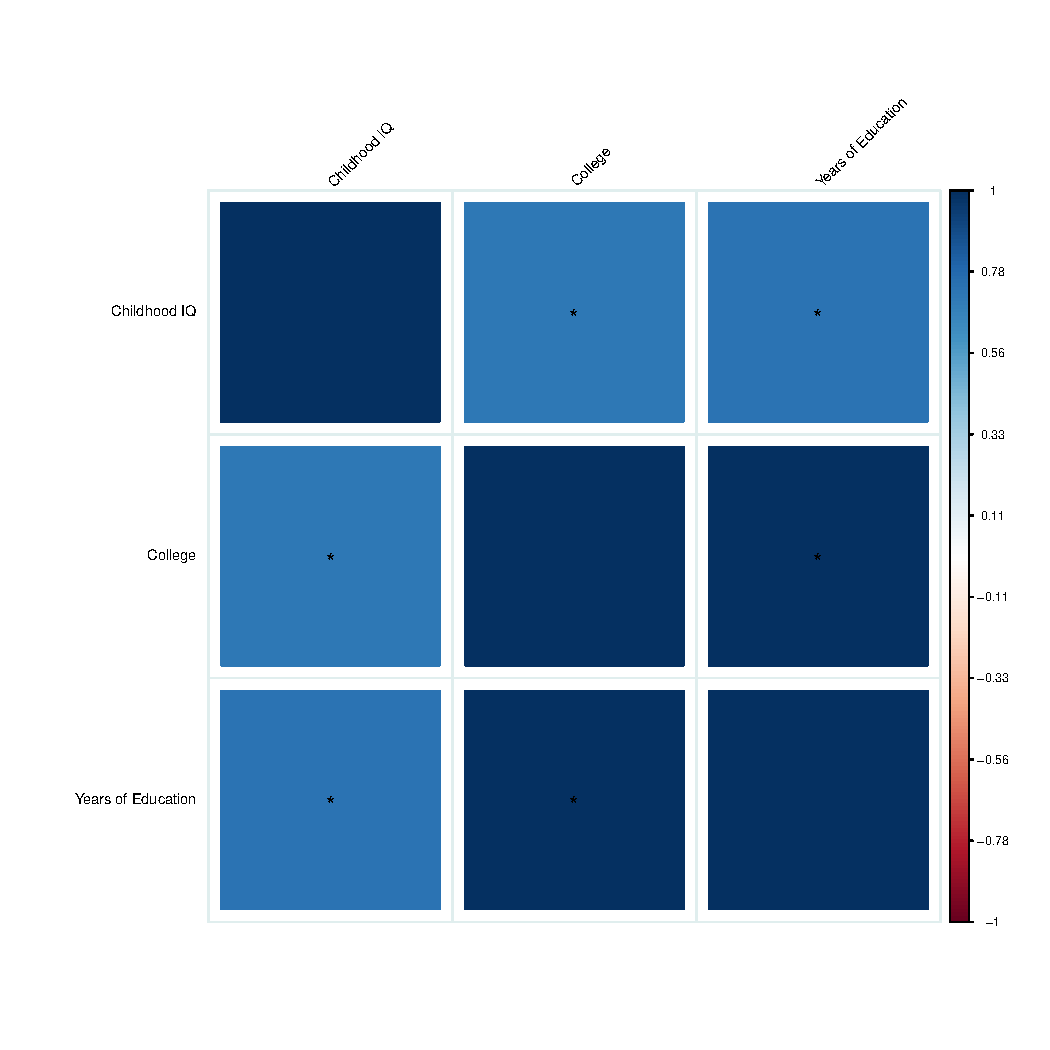
\includegraphics[scale=0.9]{figs/iq.pdf}
\caption{\label{edu}\small{Genetic correlation between the two educational attainment phenotypes from Rietveld, et al. \cite{rietveld2013gwas} and childhood IQ from \cite{benyamin2014childhood}.
The structure of the figure is the same as Figure \ref{Fig:300 Gencors} in the main text: 
blue corresponds to positive genetic correlations; red corresponds to negative genetic correlation. 
Larger squares correspond to more significant $p$-values.
Genetic correlations that are different from zero at 1\% FDR are shown as full-sized squares. 
Genetic correlations that are significantly different from zero at significance level 0.05 after Bonferroni correction are given an asterisk.}}
\end{centering}
\end{figure}
\newpage

\subsection*{Genetic Correlations among Anthropometric Traits}
\begin{figure}[!ht]
\begin{centering}
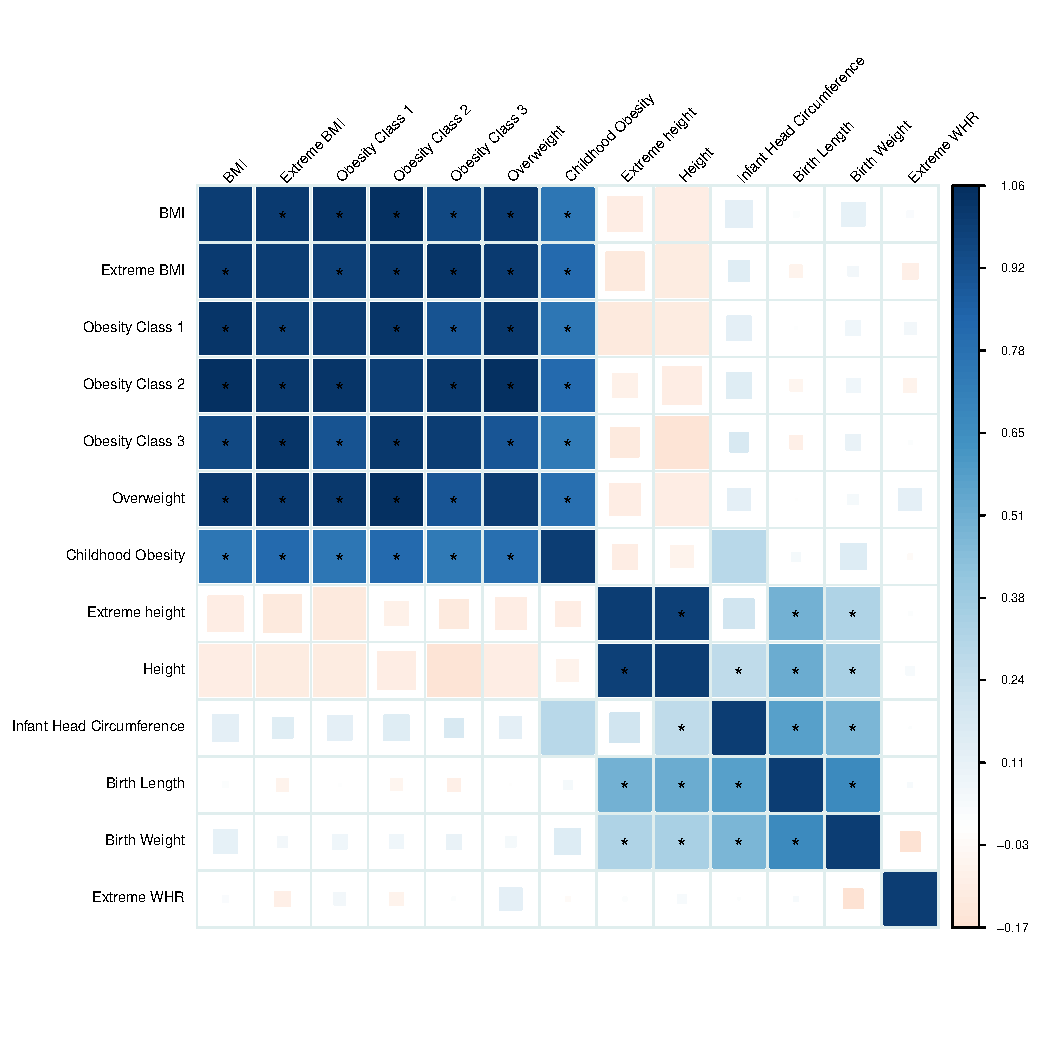
\includegraphics[scale=0.9]{figs/giant_supp.pdf}
\caption{\label{giant}\small{Genetic correlations among anthropometric traits from studies by the GIANT and EGG consortia. The structure of the figure is the same as Figure \ref{Fig:300 Gencors} in the main text: 
blue corresponds to positive genetic correlations; red corresponds to negative genetic correlation. 
Larger squares correspond to more significant $p$-values.
Genetic correlations that are different from zero at 1\% FDR are shown as full-sized squares. 
Genetic correlations that are significantly different from zero at significance level 0.05 after Bonferroni correction are given an asterisk.
BMI 2010 and Height 2010 refer to the results from \cite{speliotes2010association} and \cite{allen2010hundreds}, respectively.}}
\end{centering}
\end{figure}
\newpage

\subsection*{Genetic Correlations among Smoking Traits}
\begin{figure}[!ht]
\begin{centering}
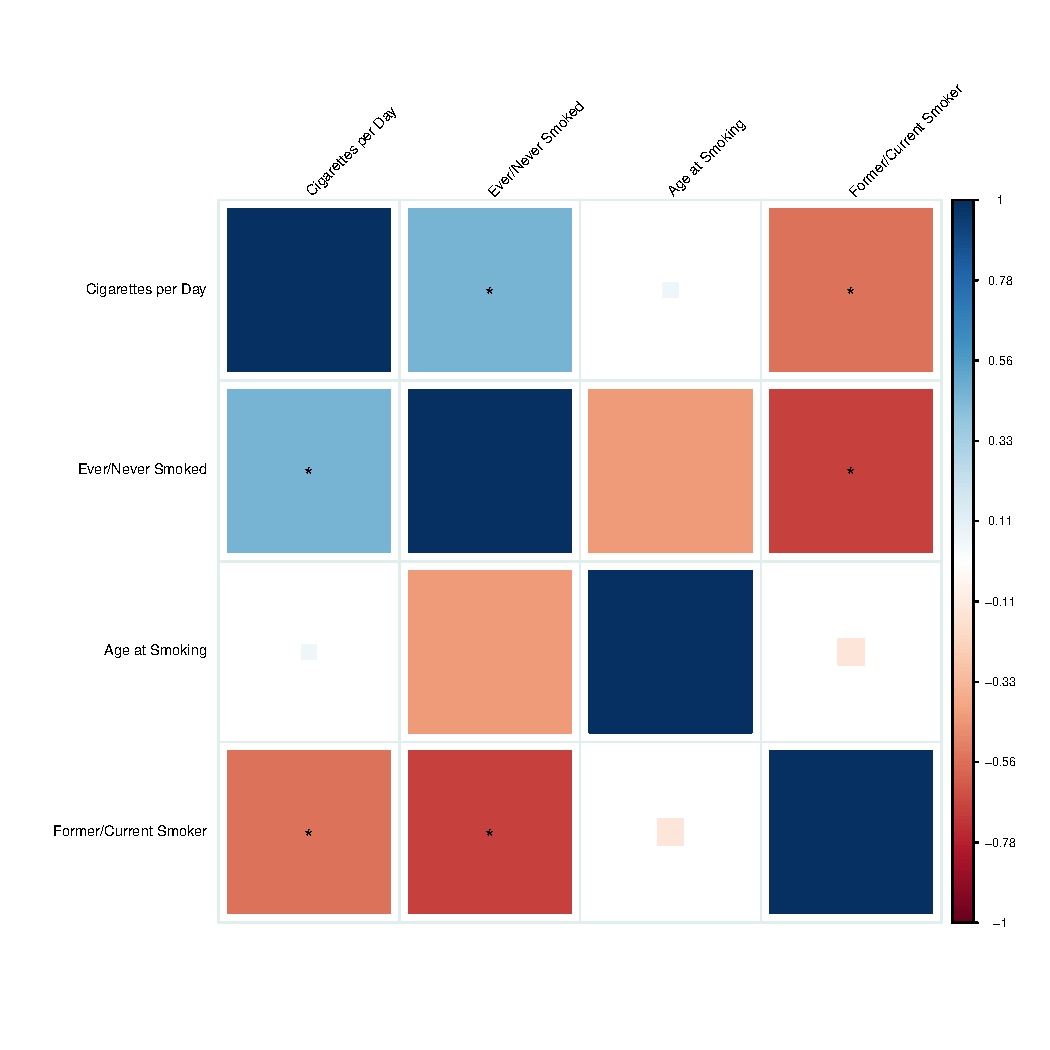
\includegraphics[scale=0.9]{figs/tag_supp.pdf}
\caption{\label{smoking}\small{Genetic correlations among smoking traits from the Tobacco and Genetics (TAG) consortium
 \cite{tobacco2010genome}. The structure of the figure is the same as Figure \ref{Fig:300 Gencors} in the main text: 
blue corresponds to positive genetic correlations; red corresponds to negative genetic correlation. 
Larger squares correspond to more significant $p$-values.
Genetic correlations that are different from zero at 1\% FDR are shown as full-sized squares. 
Genetic correlations that are significantly different from zero at significance level 0.05 after Bonferroni correction are given an asterisk.}}
\end{centering}
\end{figure}
\newpage

\subsection*{Genetic Correlations among Glycemic Traits}
\begin{figure}[!ht]
\begin{centering}
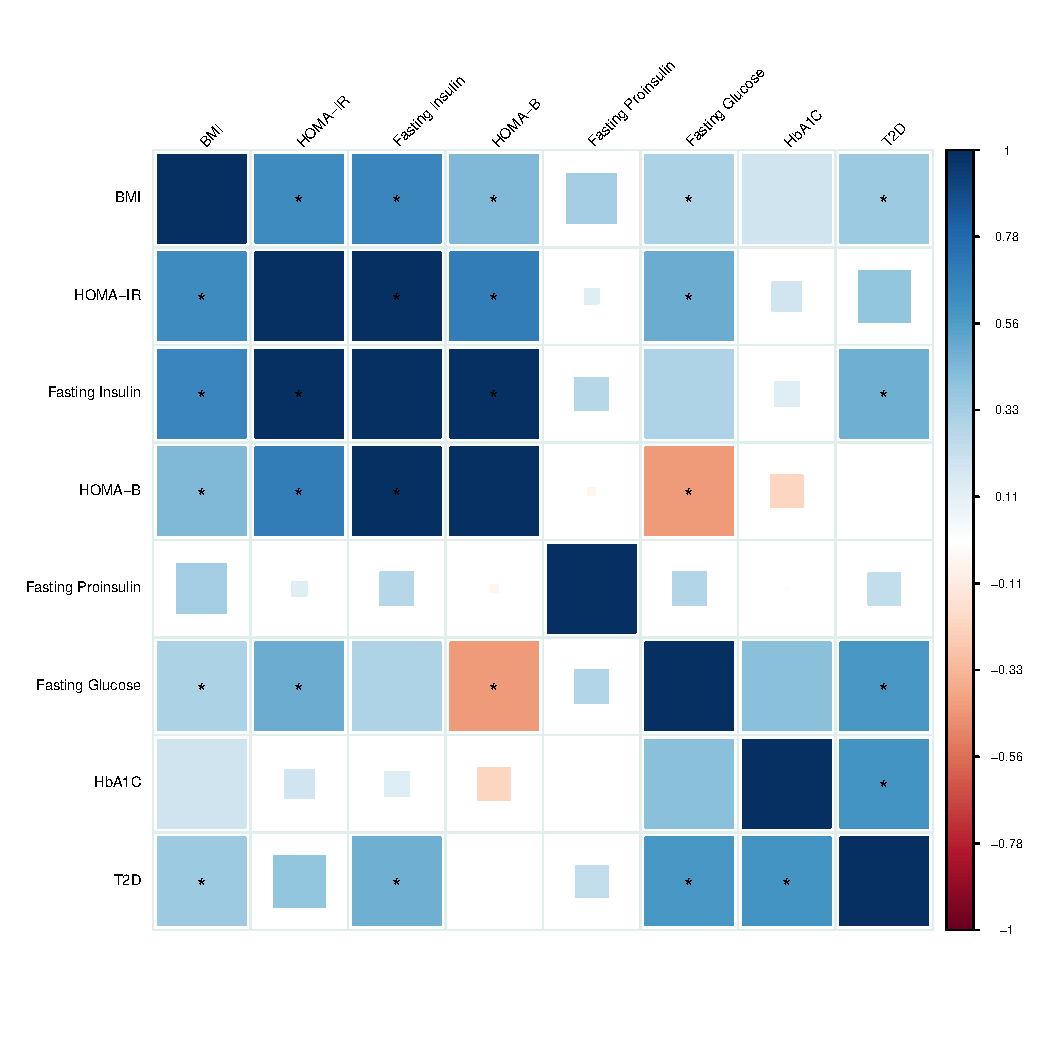
\includegraphics[scale=0.9]{figs/magic_supp.pdf}
\caption{\label{insulin}\small{Genetic correlations among insulin-related traits from studies by the MAGIC consortium. 
We have also included BMI data from \cite{locke2015genetic} and T2D data from \cite{morris2012large}.
The structure of the figure is the same as Figure \ref{Fig:300 Gencors} in the main text: 
blue corresponds to positive genetic correlations; red corresponds to negative genetic correlation. 
Larger squares correspond to more significant $p$-values.
Genetic correlations that are different from zero at 1\% FDR are shown as full-sized squares. 
Genetic correlations that are significantly different from zero at significance level 0.05 after Bonferroni correction are given an asterisk.}}
\end{centering}
\end{figure}
\newpage


\subsection*{Metabolic Genetic Correlations from Vattikuti, et al. and LD Score}
\begin{figure}[!ht]
\begin{centering}
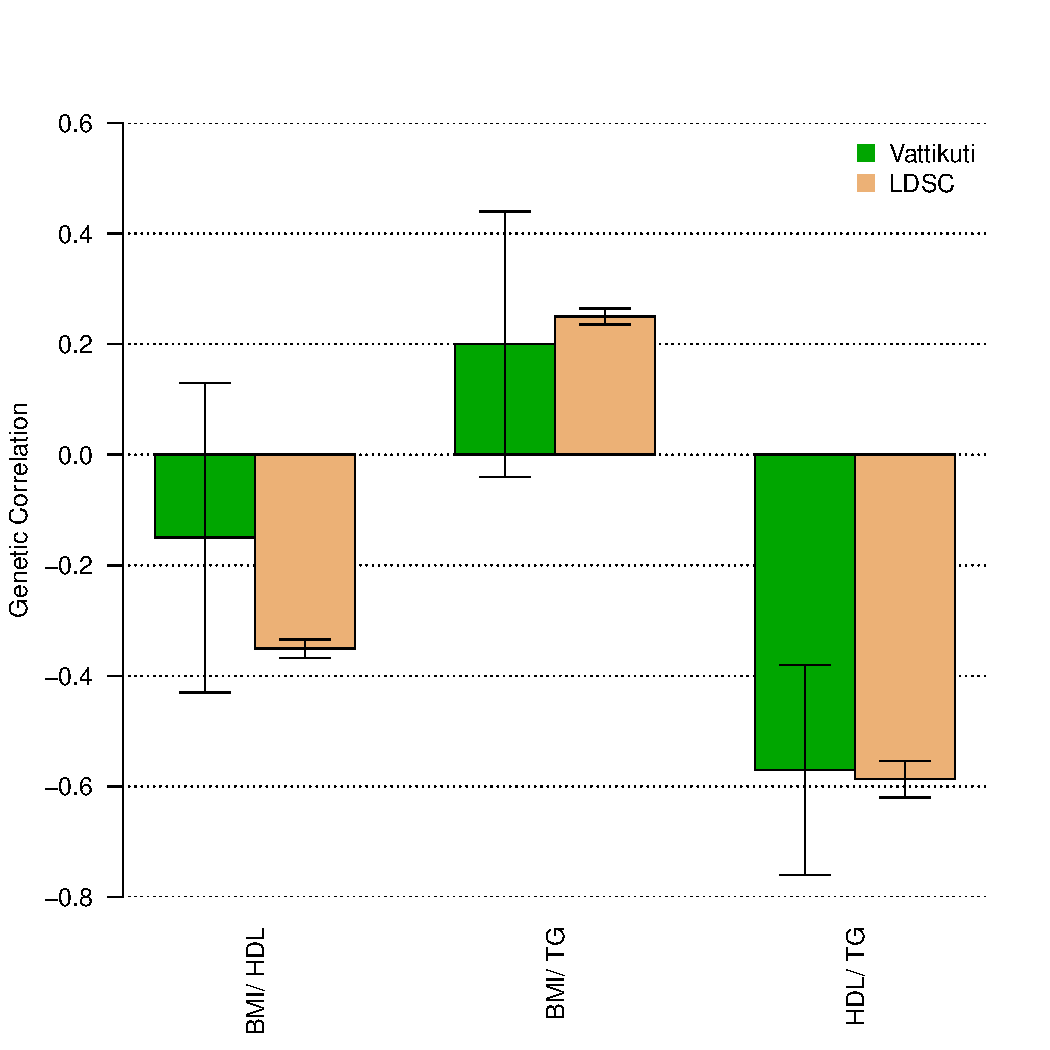
\includegraphics[scale=0.8]{figs/vattikuti.pdf}
\caption{\label{vattikuti}\small{This figure compares estimates of genetic correlations among metabolic traits from table 3 of Vattikuti et al. \cite{vattikuti2012heritability}
to estimates from LD Score regression. The LD Score regression estimates used much larger sample sizes. Error bars are standard errors.}}
\end{centering}
\end{figure}
\newpage

\subsection*{Schizophrenia | TG Conditional QQ Plot with and without the MHC}
\begin{figure}[!ht]
\begin{centering}
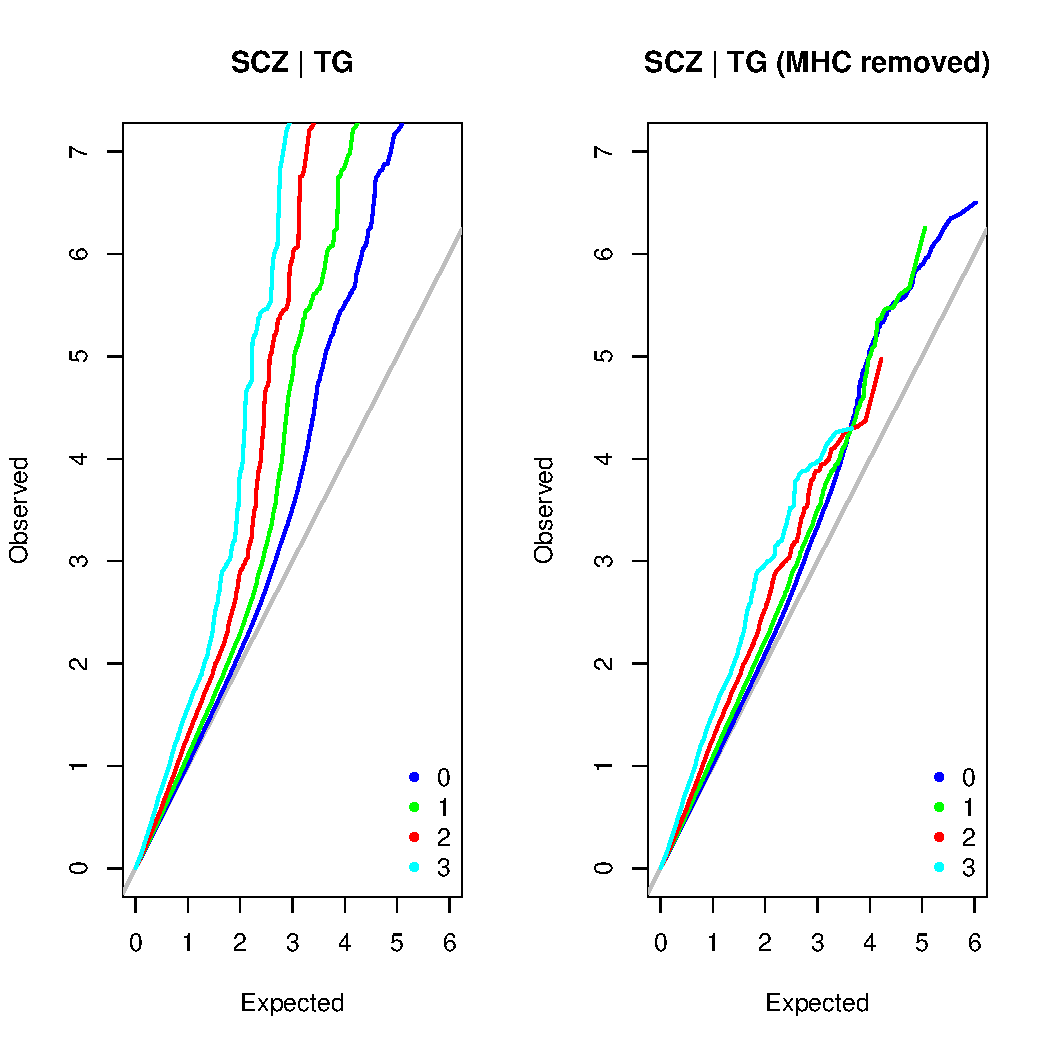
\includegraphics[scale=0.8]{figs/PGC1_pleiotropy_filter.png}
\caption{\label{qq_tg}\small{At left, we reproduced the conditional QQ plot comparing schizophrenia (SCZ) and triglycerides (TG) from Andreassen et al. \cite{andreassen2013improved2} 
using the same data (PGC1 schizophrenia \cite{schizophrenia2011genome} and TG from Teslovich, et al. \cite{teslovich2010biological}). 
Conditional QQ plots show the distribution of $p$-values for SCZ conditional on the $-\log_{10}(p)$ for TG exceeding different thresholds.
The thresholds are indicated by color, as described in the legends.
Dark blue corresponds to no threshold, green corresponds to $-\log_{10}(p)>1$, 
red corresponds to $-\log_{10}(p)>2$ and light blue corresponds to $-\log_{10}(p)>3$.
The major histocompatibility complex (MHC, chr6, 25-35 MB) is
a genomic region containing SNPs with exceptionally long-range LD and the strongest GWAS association for schizophrenia
\cite{schizophrenia2014biological}, as well as an association to TG \cite{teslovich2010biological}.
If we remove the MHC, the signal of enrichment in the conditional QQ plot is substantially attenuated (middle); in particular, the red line falls below the green and blue lines (which correspond to less stringent thresholds for TG).
If in addition we remove SNPs with very high LD Scores ($\ell>200$, roughly the top 15\% of SNPs), the signal of enrichment is further attenuated.
The most likely explanation for the attenuation is that conditional QQ plots will report pleiotropy if causal SNPs are in LD (even if the causal SNPs for trait 1 are different from the causal SNPs for trait 2),
which is more likely to occur in regions with long-range LD.}}
\end{centering}
\end{figure}
\newpage

%%%%%%%%%%%%%%%%%%%%%%%%%%%%%%%%%%%%%%%%%%%%%%%%%%%%%%%%%%%%%%%
\section*{Collaborators}
%%%%%%%%%%%%%%%%%%%%%%%%%%%%%%%%%%%%%%%%%%%%%%%%%%%%%%%%%%%%%%%

Collaborators from the Psychiatric Genomics Consortium were, in
alphabetical order: Devin Absher, Rolf Adolfsson, Ingrid Agartz, Esben
Agerbo, Huda Akil, Margot Albus, Madeline Alexander, Farooq Amin, Ole A
Andreassen, Adebayo Anjorin, Richard Anney, Dan Arking, Philip Asherson,
Maria H Azevedo, Silviu A Bacanu, Lena Backlund, Judith A Badner, Tobias
Banaschewski, Jack D Barchas, Michael R Barnes, Thomas B Barrett,
Nicholas Bass, Michael Bauer, Monica Bayes, Martin Begemann, Frank
Bellivier, Judit Bene, Sarah E Bergen, Thomas Bettecken, Elizabeth
Bevilacqua, Joseph Biederman, Tim B Bigdeli, Elisabeth B Binder, Donald
W Black, Douglas HR Blackwood, Cinnamon S Bloss, Michael Boehnke, Dorret
I Boomsma, Anders D Borglum, Elvira Bramon, Gerome Breen, Rene Breuer,
Richard Bruggeman, Nancy G Buccola, Randy L Buckner, Jan K Buitelaar,
Brendan Bulik-Sullivan, William E Bunner, Margit Burmeister, Joseph D
Buxbaum, William F Byerley, Sian Caesar, Wiepke Cahn, Guiqing Cai,
Murray J Cairns, Dominique Campion, Rita M Cantor, Vaughan J Carr, Noa
Carrera, Miquel Casas, Stanley V Catts, Aravinda Chakravarti, Kimberley
D Chambert, Raymond CK Chan, Eric YH Chen, Ronald YL Chen, Wei Cheng,
Eric FC Cheung, Siow Ann Chong, Khalid Choudhury, Sven Cichon, David St
Clair, C Robert Cloninger, David Cohen, Nadine Cohen, David A Collier,
Edwin Cook, Hilary Coon, Bru Cormand, Paul Cormican, Aiden Corvin,
William H Coryell, Nicholas Craddock, David W Craig, Ian W Craig,
Benedicto Crespo-Facorro, James J Crowley, David Curtis, Darina Czamara,
Mark J Daly, Ariel Darvasi, Susmita Datta, Michael Davidson, Kenneth L
Davis, Richard Day, Franziska Degenhardt, Lynn E DeLisi, Ditte Demontis,
Bernie Devlin, Dimitris Dikeos, Timothy Dinan, Srdjan Djurovic, Enrico
Domenici, Gary Donohoe, Alysa E Doyle, Elodie Drapeau, Jubao Duan, Frank
Dudbridge, Naser Durmishi, Howard J Edenberg, Hannelore Ehrenreich,
Peter Eichhammer, Amanda Elkin, Johan Eriksson, Valentina Escott-Price,
Tonu Esko, Laurent Essioux, Bruno Etain, Ayman H Fanous, Stephen V
Faraone, Kai-How Farh, Anne E Farmer, Martilias S Farrell, Jurgen Del
Favero, Manuel A Ferreira, I Nicol Ferrier, Matthew Flickinger, Tatiana
Foroud, Josef Frank, Barbara Franke, Lude Franke, Christine Fraser,
Robert Freedman, Nelson B Freimer, Marion Friedl, Joseph I Friedman,
Louise Frisen, Menachem Fromer, Pablo V Gejman, Giulio Genovese,
Lyudmila Georgieva, Elliot S Gershon, Eco J De Geus, Ina Giegling,
Michael Gill, Paola Giusti-Rodriguez, Stephanie Godard, Jacqueline I
Goldstein, Vera Golimbet, Srihari Gopal, Scott D Gordon, Katherine
Gordon-Smith, Jacob Gratten, Elaine K Green, Tiffany A Greenwood, Gerard
Van Grootheest, Magdalena Gross, Detelina Grozeva, Weihua Guan, Hugh
Gurling, Omar Gustafsson, Lieuwe de Haan, Hakon Hakonarson, Steven P
Hamilton, Christian Hammer, Marian L Hamshere, Mark Hansen, Thomas F
Hansen, Vahram Haroutunian, Annette M Hartmann, Martin Hautzinger,
Andrew C Heath, Anjali K Henders, Frans A Henskens, Stefan Herms, Ian B
Hickie, Maria Hipolito, Joel N Hirschhorn, Susanne Hoefels, Per
Hoffmann, Andrea Hofman, Mads V Hollegaard, Peter A Holmans, Florian
Holsboer, Witte J Hoogendijk, Jouke Jan Hottenga, David M Hougaard,
Hailiang Huang, Christina M Hultman, Masashi Ikeda, Andres Ingason,
Marcus Ising, Nakao Iwata, Assen V Jablensky, Stephane Jamain, Inge Joa,
Edward G Jones, Ian Jones, Lisa Jones, Erik G Jonsson, Milan Macek Jr,
Richard A Belliveau Jr, Antonio Julia, Tzeng Jung-Ying, Anna K Kahler,
Rene S Kahn, Luba Kalaydjieva, Radhika Kandaswamy, Sena
Karachanak-Yankova, Juha Karjalainen, David Kavanagh, Matthew C Keller,
Brian J Kelly, John R Kelsoe, Kenneth S Kendler, James L Kennedy, Elaine
Kenny, Lindsey Kent, Jimmy Lee Chee Keong, Andrey Khrunin, Yunjung Kim,
George K Kirov, Janis Klovins, Jo Knight, James A Knowles, Martin A
Kohli, Daniel L Koller, Bettina Konte, Ania Korszun, Robert Krasucki,
Vaidutis Kucinskas, Zita Ausrele Kucinskiene, Jonna Kuntsi, Hana
Kuzelova-Ptackova, Phoenix Kwan, Mikael Landen, Niklas Langstrom, Mark
Lathrop, Claudine Laurent, Jacob Lawrence, William B Lawson, Marion
Leboyer, Phil Hyoun Lee, S Hong Lee, Sophie E Legge, Todd Lencz, Bernard
Lerer, Klaus-Peter Lesch, Douglas F Levinson, Cathryn M Lewis, Jun Li,
Miaoxin Li, Qingqin S Li, Tao Li, Kung-Yee Liang, Paul Lichtenstein,
Jeffrey A Lieberman, Svetlana Limborska, Danyu Lin, Chunyu Liu, Jianjun
Liu, Falk W Lohoff, Jouko Lonnqvist, Sandra K Loo, Carmel M Loughland,
Jan Lubinski, Susanne Lucae, Donald MacIntyre, Pamela AF Madden, Patrik
KE Magnusson, Brion S Maher, Pamela B Mahon, Wolfgang Maier, Anil K
Malhotra, Jacques Mallet, Sara Marsal, Nicholas G Martin, Manuel
Mattheisen, Keith Matthews, Morten Mattingsdal, Robert W McCarley,
Steven A McCarroll, Colm McDonald, Kevin A McGhee, James J McGough,
Patrick J McGrath, Peter McGuffin, Melvin G McInnis, Andrew M McIntosh,
Rebecca McKinney, Alan W McLean, Francis J McMahon, Andrew McQuillin,
Helena Medeiros, Sarah E Medland, Sandra Meier, Carin J Meijer, Bela
Melegh, Ingrid Melle, Fan Meng, Raquelle I Mesholam-Gately, Andres
Metspalu, Patricia T Michie, Christel M Middeldorp, Lefkos Middleton,
Lili Milani, Vihra Milanova, Philip B Mitchell, Younes Mokrab, Grant W
Montgomery, Jennifer L Moran, Gunnar Morken, Derek W Morris, Ole Mors,
Preben B Mortensen, Valentina Moskvina, Bryan J Mowry, Pierandrea
Muglia, Thomas W Muehleisen, Walter J Muir, Bertram Mueller-Myhsok, Kieran
C Murphy, Robin M Murray, Richard M Myers, Inez Myin-Germeys, Benjamin M
Neale, Michael C Neale, Mari Nelis, Stan F Nelson, Igor Nenadic, Deborah
A Nertney, Gerald Nestadt, Kristin K Nicodemus, Caroline M Nievergelt,
Liene Nikitina-Zake, Ivan Nikolov, Vishwajit Nimgaonkar, Laura
Nisenbaum, Willem A Nolen, Annelie Nordin, Markus M Noethen, John I
Nurnberger, Evaristus A Nwulia, Dale R Nyholt, Eadbhard O'Callaghan,
Michael C O'Donovan, Colm O'Dushlaine, F Anthony O'Neill, Robert D
Oades, Sang-Yun Oh, Ann Olincy, Line Olsen, Edwin JCG van den Oord, Roel
A Ophoff, Jim Van Os, Urban Osby, Hogni Oskarsson, Michael J Owen, Aarno
Palotie, Christos Pantelis, George N Papadimitriou, Sergi Papiol, Elena
Parkhomenko, Carlos N Pato, Michele T Pato, Tiina Paunio, Milica
Pejovic-Milovancevic, Brenda P Penninx, Michele L Pergadia, Diana O
Perkins, Roy H Perlis, Tune H Pers, Tracey L Petryshen, Hannes
Petursson, Benjamin S Pickard, Olli Pietilainen, Jonathan Pimm, Joseph
Piven, Andrew J Pocklington, Porgeir Porgeirsson, Danielle Posthuma,
James B Potash, John Powell, Alkes Price, Peter Propping, Ann E Pulver,
Shaun M Purcell, Vinay Puri, Digby Quested, Emma M Quinn, Josep Antoni
Ramos-Quiroga, Henrik B Rasmussen, Soumya Raychaudhuri, Karola
Rehnstrom, Abraham Reichenberg, Andreas Reif, Mark A Reimers, Marta
Ribases, John Rice, Alexander L Richards, Marcella Rietschel, Brien P
Riley, Stephan Ripke, Joshua L Roffman, Lizzy Rossin, Aribert
Rothenberger, Guy Rouleau, Panos Roussos, Douglas M Ruderfer, Dan
Rujescu, Veikko Salomaa, Alan R Sanders, Susan Santangelo, Russell
Schachar, Ulrich Schall, Martin Schalling, Alan F Schatzberg, William A
Scheftner, Gerard Schellenberg, Peter R Schofield, Nicholas J Schork,
Christian R Schubert, Thomas G Schulze, Johannes Schumacher, Sibylle G
Schwab, Markus M Schwarz, Edward M Scolnick, Laura J Scott, Rodney J
Scott, Larry J Seidman, Pak C Sham, Jianxin Shi, Paul D Shilling,
Stanley I Shyn, Engilbert Sigurdsson, Teimuraz Silagadze, Jeremy M
Silverman, Kang Sim, Pamela Sklar, Susan L Slager, Petr Slominsky, Susan
L Smalley, Johannes H Smit, Erin N Smith, Jordan W Smoller, Hon-Cheong
So, Erik Soderman, Edmund Sonuga-Barke, Chris C A Spencer, Eli A Stahl,
Matthew State, Hreinn Stefansson, Kari Stefansson, Michael Steffens,
Stacy Steinberg, Hans-Christoph Steinhausen, Elisabeth Stogmann, Richard
E Straub, John Strauss, Eric Strengman, Jana Strohmaier, T Scott Stroup,
Mythily Subramaniam, Patrick F Sullivan, James Sutcliffe, Jaana
Suvisaari, Dragan M Svrakic, Jin P Szatkiewicz, Peter Szatmari, Szabocls
Szelinger, Anita Thapar, Srinivasa Thirumalai, Robert C Thompson, Draga
Toncheva, Paul A Tooney, Sarah Tosato, Federica Tozzi, Jens Treutlein,
Manfred Uhr, Juha Veijola, Veronica Vieland, John B Vincent, Peter M
Visscher, John Waddington, Dermot Walsh, James TR Walters, Dai Wang,
Qiang Wang, Stanley J Watson, Bradley T Webb, Daniel R Weinberger, Mark
Weiser, Myrna M Weissman, Jens R Wendland, Thomas Werge, Thomas F
Wienker, Dieter B Wildenauer, Gonneke Willemsen, Nigel M Williams,
Stephanie Williams, Richard Williamson, Stephanie H Witt, Aaron R Wolen,
Emily HM Wong, Brandon K Wormley, Naomi R Wray, Adam Wright, Jing Qin
Wu, Hualin Simon Xi, Wei Xu, Allan H Young, Clement C Zai, Stan Zammit,
Peter P Zandi, Peng Zhang, Xuebin Zheng, Fritz Zimprich, Frans G Zitman,
and Sebastian Zoellner. 

Genetic Consortium for Anorexia Nervosa (GCAN):
Vesna Boraska Perica, Christopher S Franklin, James A B Floyd, Laura M Thornton, Laura M Huckins, Lorraine Southam, N William Rayner, Ioanna Tachmazidou, Kelly L Klump, Janet Treasure, Cathryn M Lewis, Ulrike Schmidt, Federica Tozzi, Kirsty Kiezebrink, Johannes Hebebrand, Philip Gorwood, Roger A H Adan, Martien J H Kas, Angela Favaro, Paolo Santonastaso, Fernando Fern\'{a}ndez-Aranda, Monica Gratacos, Filip Rybakowski, Monika Dmitrzak-Weglarz, Jaakko Kaprio, Anna Keski-Rahkonen, Anu Raevuori-Helkamaa, Eric F Van Furth, Margarita C T Slof-Op't Landt, James I Hudson, Ted Reichborn-Kjennerud, Gun Peggy S Knudsen, Palmiero Monteleone, Allan S Kaplan, Andreas Karwautz, Hakon Hakonarson, Wade H Berrettini, Yiran Guo, Dong Li, Nicholas J Schork, Gen Komaki, Tetsuya Ando, Hidetoshi Inoko, T\~{o}nu Esko, Krista Fischer, Katrin M\"{a}nnik, Andres Metspalu, Jessica H Baker, Roger D Cone, Jennifer Dackor, Janiece E DeSocio, Christopher E Hilliard, Julie K O'Toole, Jacques Pantel, Jin P Szatkiewicz, Chrysecolla Taico, Stephanie Zerwas, Sara E Trace, Oliver S P Davis, Sietske Helder, Katharina B\"{u}hren, Roland Burghardt, Martina de Zwaan, Karin Egberts, Stefan Ehrlich, Beate Herpertz-Dahlmann, Wolfgang Herzog, Hartmut Imgart, Andr\'{e} Scherag, Susann Scherag, Stephan Zipfel, Claudette Boni, Nicolas Ramoz, Audrey Versini, Marek K Brandys, Unna N Danner, Carolien de Kove, Judith Hendriks, Bobby P C Koeleman, Roel A Ophoff, Eric Strengman, Annemarie A van Elburg, Alice Bruson, Maurizio Clementi, Daniela Degortes, Monica Forzan, Elena Tenconi, Elisa Docampo, Ge\`{o}rgia Escaram\'{i}, Susana Jim\'{e}nez-Murcia, Jolanta Lissowska, Andrzej Rajewski, Neonila Szeszenia-Dabrowska, Agnieszka Slopien, Joanna Hauser, Leila Karhunen, Ingrid Meulenbelt, P Eline Slagboom, Alfonso Tortorella, Mario Maj, George Dedoussis, Dimitris Dikeos, Fragiskos Gonidakis, Konstantinos Tziouvas, Artemis Tsitsika, Hana Papezova, Lenka Slachtova, Debora Martaskova, James L Kennedy, Robert D Levitan, Zeynep Yilmaz, Julia Huemer, Doris Koubek, Elisabeth Merl, Gudrun Wagner, Paul Lichtenstein, Gerome Breen, Sarah Cohen-Woods, Anne Farmer, Peter McGuffin, Sven Cichon, Ina Giegling, Stefan Herms, Dan Rujescu, Stefan Schreiber, H-Erich Wichmann, Christian Dina, Rob Sladek, Giovanni Gambaro, Nicole Soranzo, Antonio Julia, Sara Marsal, Raquel Rabionet, Valerie Gaborieau, Danielle M Dick, Aarno Palotie, Samuli Ripatti, Elisabeth Wid\'{e}n, Ole A Andreassen, Thomas Espeseth, Astri Lundervold, Ivar Reinvang, Vidar M Steen, Stephanie Le Hellard, Morten Mattingsdal, Ioanna Ntalla, Vladimir Bencko, Lenka Foretova, Vladimir Janout, Marie Navratilova, Steven Gallinger, Dalila Pinto, Stephen W Scherer, Harald Aschauer, Laura Carlberg, Alexandra Schosser, Lars Alfredsson, Bo Ding, Lars Klareskog, Leonid Padyukov, Chris Finan, Gursharan Kalsi, Marion Roberts, Darren W Logan, Leena Peltonen, Graham R S Ritchie, Jeff C Barrett, Xavier Estivill, Anke Hinney, Patrick F Sullivan, David A Collier, Eleftheria Zeggini, and Cynthia M Bulik.

Wellcome Trust Case Control Consortium 3 (WTCCC3):
Carl A Anderson, Jeffrey C Barrett, James A B Floyd, Christopher S Franklin, Ralph McGinnis, Nicole Soranzo, Eleftheria Zeggini, Jennifer Sambrook, Jonathan Stephens, Willem H Ouwehand, Wendy L McArdle, Susan M Ring, David P Strachan, Graeme Alexander, Cynthia M Bulik, David A Collier, Peter J Conlon, Anna Dominiczak, Audrey Duncanson, Adrian Hill, Cordelia Langford, Graham Lord, Alexander P Maxwell, Linda Morgan, Leena Peltonen, Richard N Sandford, Neil Sheerin, Frederik O Vannberg, Hannah Blackburn, Wei-Min Chen, Sarah Edkins, Mathew Gillman, Emma Gray, Sarah E Hunt, Suna Nengut-Gumuscu, Simon Potter, Stephen S Rich, Douglas Simpkin, and Pamela Whittaker.

The members of the ReproGen consortium are John RB Perry, Felix Day, Cathy E Elks, Patrick Sulem, Deborah J Thompson, Teresa Ferreira, Chunyan He, Daniel I Chasman, T�nu Esko, Gudmar Thorleifsson, Eva Albrecht, Wei Q Ang, Tanguy Corre, Diana L Cousminer, Bjarke Feenstra, Nora Franceschini, Andrea Ganna, Andrew D Johnson, Sanela Kjellqvist, Kathryn L Lunetta, George McMahon, Ilja M Nolte, Lavinia Paternoster, Eleonora Porcu, Albert V Smith, Lisette Stolk, Alexander Teumer, Natalia T�ernikova, Emmi Tikkanen, Sheila Ulivi, Erin K Wagner, Najaf Amin, Laura J Bierut, Enda M Byrne, JoukeJan Hottenga, Daniel L Koller, Massimo Mangino, Tune H Pers, Laura M YergesArmstrong, Jing Hua Zhao, Irene L Andrulis, Hoda AntonCulver, Femke Atsma, Stefania Bandinelli, Matthias W Beckmann, Javier Benitez, Carl Blomqvist, Stig E Bojesen, Manjeet K Bolla, Bernardo Bonanni, Hiltrud Brauch, Hermann Brenner, Julie E Buring, Jenny ChangClaude, Stephen Chanock, Jinhui Chen, Georgia ChenevixTrench, J. Margriet Coll�e, Fergus J Couch, David Couper, Andrea D Coveillo, Angela Cox, Kamila Czene, Adamo Pio D'adamo, George Davey Smith, Immaculata De Vivo, Ellen W Demerath, Joe Dennis, Peter Devilee, Aida K Dieffenbach, Alison M Dunning, Gudny Eiriksdottir, Johan G Eriksson, Peter A Fasching, Luigi Ferrucci, Dieter FleschJanys, Henrik Flyger, Tatiana Foroud, Lude Franke, Melissa E Garcia, Montserrat Garc�aClosas, Frank Geller, Eco EJ de Geus, Graham G Giles, Daniel F Gudbjartsson, Vilmundur Gudnason, Pascal Gu�nel, Suiqun Guo, Per Hall, Ute Hamann, Robin Haring, Catharina A Hartman, Andrew C Heath, Albert Hofman, Maartje J Hooning, John L Hopper, Frank B Hu, David J Hunter, David Karasik, Douglas P Kiel, Julia A Knight, VeliMatti Kosma, Zoltan Kutalik, Sandra Lai, Diether Lambrechts, Annika Lindblom, Reedik M�gi, Patrik K Magnusson, Arto Mannermaa, Nicholas G Martin, Gisli Masson, Patrick F McArdle, Wendy L McArdle, Mads Melbye Kyriaki Michailidou, Evelin Mihailov, Lili Milani, Roger L Milne, Heli Nevanlinna, Patrick Neven, Ellen A Nohr, Albertine J Oldehinkel, Ben A Oostra, Aarno Palotie,, Munro Peacock, Nancy L Pedersen, Paolo Peterlongo, Julian Peto, Paul DP Pharoah, Dirkje S Postma, Anneli Pouta, Katri Pylk�s, Paolo Radice, Susan Ring, Fernando Rivadeneira, Antonietta Robino, Lynda M Rose, Anja Rudolph, Veikko Salomaa, Serena Sanna, David Schlessinger, Marjanka K Schmidt, Mellissa C Southey, Ulla Sovio Meir J Stampfer, Doris St�ckl Anna M Storniolo, Nicholas J Timpson Jonathan Tyrer, Jenny A Visser, Peter Vollenweider, Henry V�lzke, Gerard Waeber, Melanie Waldenberger, Henri Wallaschofski, Qin Wang, Gonneke Willemsen, Robert Winqvist, Bruce HR Wolffenbuttel, Margaret J Wright, Australian Ovarian Cancer Study The GENICA Network, kConFab, The LifeLines Cohort Study, The InterAct Consortium, Early Growth Genetics (EGG) Consortium, Dorret I Boomsma, Michael J Econs, KayTee Khaw, Ruth JF Loos, Mark I McCarthy, Grant W Montgomery, John P Rice, Elizabeth A Streeten, Unnur Thorsteinsdottir, Cornelia M van Duijn, Behrooz Z Alizadeh, Sven Bergmann, Eric Boerwinkle, Heather A Boyd, Laura Crisponi, Paolo Gasparini, Christian Gieger, Tamara B Harris, Erik Ingelsson, MarjoRiitta J�rvelin, Peter Kraft, Debbie Lawlor, Andres Metspalu, Craig E Pennell, Paul M Ridker, Harold Snieder, Thorkild IA S�rensen, Tim D Spector, David P Strachan, Andr� G Uitterlinden, Nicholas J Wareham, Elisabeth Widen, Marek Zygmunt, Anna Murray, Douglas F Easton, Kari Stefansson, Joanne M Murabito, Ken K Ong.
\end{document}
